\documentclass[11pt,a4paper]{article}
\usepackage[T1]{fontenc}
\usepackage[utf8]{inputenc}
\usepackage{amsmath,amsthm}
\usepackage{newtxtext,newtxmath}
\usepackage[margin=26mm,headheight=14pt]{geometry}
\usepackage{microtype}
\usepackage{mathtools,bm}
\usepackage{booktabs,longtable,tabularx,array}
\usepackage{graphicx,float}
\usepackage{enumitem}
\usepackage{xurl}
\usepackage[hidelinks]{hyperref}
\hypersetup{
 pdftitle={Three Exceptions Before Every Square},
 pdfauthor={Research report prepared for Vladimir Reshetnikov},
 pdfsubject={Sharp asymptotics and inverse expansions for OEIS A097356 and related partitions},
 pdfkeywords={OEIS, A097356, restricted partitions, saddle point, asymptotic expansion, inversion}
}
\usepackage[nameinlink,noabbrev]{cleveref}
\usepackage{fancyhdr}
\usepackage{listings}
\usepackage{caption}
\captionsetup{font=small,labelfont=bf}
\pagestyle{fancy}
\fancyhf{}
\fancyhead[L]{\small Square-root-restricted partitions}
\fancyhead[R]{\small OEIS research report}
\fancyfoot[C]{\thepage}
\setlength{\parskip}{3pt}
\setlength{\parindent}{1.25em}
\setlength{\emergencystretch}{2em}
\setcounter{tocdepth}{2}
\numberwithin{equation}{section}
\newtheorem{theorem}{Theorem}[section]
\newtheorem{lemma}[theorem]{Lemma}
\newtheorem{proposition}[theorem]{Proposition}
\newtheorem{corollary}[theorem]{Corollary}
\theoremstyle{definition}
\newtheorem{definition}[theorem]{Definition}
\theoremstyle{remark}
\newtheorem{remark}[theorem]{Remark}
\DeclareMathOperator{\Li}{Li}
\DeclareMathOperator{\dist}{dist}
\newcommand{\dd}{\,\mathrm d}
\newcommand{\e}{\mathrm e}
\newcommand{\ii}{\mathrm i}
\newcommand{\N}{\mathbb N}
\newcommand{\R}{\mathbb R}
\newcommand{\C}{\mathbb C}
\newcommand{\E}{\mathcal E}
\newcommand{\G}{\mathcal G}
\newcommand{\floor}[1]{\left\lfloor #1\right\rfloor}
\newcommand{\ceil}[1]{\left\lceil #1\right\rceil}
\newcommand{\fracpart}[1]{\left\{#1\right\}}
\newcommand{\coeff}[2]{\left[#1\right]#2}
\newcommand{\oeis}[1]{\href{https://oeis.org/#1}{\texttt{#1}}}
\lstset{basicstyle=\small\ttfamily,breaklines=true,columns=fullflexible,frame=single}
% Collection edition (batch 73O1): notes added when the report was written
% into ProveIt's research-report collection.
\newcommand{\writenote}[1]{\par\smallskip\noindent
 \textit{[Write note, batch 73O1, 1 October 2026.]}\ #1\par\smallskip}
% Batch 74: notes added when manuscript 02 of batch 74 was merged.
\newcommand{\writenotefour}[1]{\par\smallskip\noindent
 \textit{[Write note, batch 74, 1 October 2026.]}\ #1\par\smallskip}

\title{\textbf{Three Exceptions Before Every Square}\\[5pt]
\large Sharp OEIS partition asymptotics, an all-orders coefficient calculus,\\
and phase-sensitive inverse transseries}
\author{Research report prepared for Vladimir Reshetnikov}
\date{October 1, 2026}

\begin{document}
\maketitle
\begin{abstract}
Let $A(N)$ count the partitions of $N$ whose parts do not exceed
$\lfloor\sqrt N\rfloor$; this is OEIS A097356. A posted conjecture identifies
$0.088154883798697116\ldots$ as its lower asymptotic constant. We prove that
this is exactly the sharp limit-inferior constant, while distinguishing that
statement from a literal lower-bound inequality. The latter is eventually
false at precisely three indices in every square block: the three integers
immediately preceding the next square.

The proof is obtained from a uniform, all-orders expansion for
$p_m(\alpha m^2+\sigma m+\tau)$, where $p_m$ counts partitions with parts at
most $m$. An explicit finite Gaussian coefficient operator generates every
correction. For A097356 the expansion has a nonvanishing phase factor
$\rho^{\{\sqrt N\}}$ and polynomial corrections. We derive its cluster set,
limiting distribution, summatory asymptotic, and inverse staircase. A
Lambert-$W_{-1}$ core suffices for the square subsequence, but the full
sequence requires an additional piecewise-linear phase map: omitting it
can cause an index error of order $\log Y$, whereas including it gives an
$O(1)$ error. The shifted quadratic sequences A206227 and A206240 are
covered by the same calculus.

The leading restricted-partition asymptotic is classical Szekeres theory,
not a new discovery here. The endpoint classification and the detailed
coefficient and inverse refinements are developed explicitly in this
report. Analytic proofs, exact rational sign certificates, and
high-precision checks are separated throughout. No complete
exponentially improved transseries, effective last exceptional block,
or machine-checked formalization is claimed.
\end{abstract}
\vspace{3pt}
\noindent\textbf{Included artifacts.} Editable \LaTeX, compiled PDF, two figures,
reproducible Python code, exact rational certificates, and numerical tables.

\writenote{This is the collection edition of the report, written into
ProveIt's research-report collection from manuscript~38 of batch~73O1
(provenance in \cref{srp:app:provenance}). Every label carries the
prefix \texttt{srp:}; the scripts now live in \texttt{code/} and the
recorded outputs of the delivered \texttt{results/} directory in
\texttt{data/}. Text added in the write is marked like this note;
everything else is the delivered text. Two readings to keep in mind:
the subtitle's word ``transseries'' is used loosely, since the expansions
are phase-parametrized Poincar\'e expansions (the paragraph ``Precise
meaning of `all orders'\,'' in \cref{srp:sec:scope} says so); and the
discrete threshold proposition, \cref{srp:prop:ceil}, is an instance of a
theorem the repository already proves (see the note after it).}

\writenotefour{A second manuscript, number~02 of batch~74, proves the
three main theorems independently and with the same constants. It is
merged as \cref{srp:se:sec:second}, after the conclusion: the shared
theorems are printed once, in their places below, with its proofs as
marked second routes, and its own results (a classical first-order route,
exact degrees, second-order envelope constants, the exact phase loss of
the uncorrected inverse, a Fourier identity) are printed there. Its rate
for the log-uniform law stands beside \cref{srp:thm:distribution}.
Provenance of both manuscripts is in \cref{srp:app:provenance}.}

\newpage
\tableofcontents
\newpage

\section{The OEIS question and the scope of the result}
\label{srp:sec:scope}

\subsection{Why this family is a worthwhile target}
The restricted partition function
\begin{equation}
 p_m(N)=[q^N]P_m(q),\qquad
 P_m(q)=\prod_{j=1}^m(1-q^j)^{-1},
 \label{srp:eq:definition}
\end{equation}
is a basic object in enumerative combinatorics. The cutoff $m\asymp\sqrt N$
is a natural two-parameter regime, not an artificially selected sparse
sequence. In particular,
\begin{equation}
 A(N)=p_{\lfloor\sqrt N\rfloor}(N)\quad(N\ge1),\qquad A(0)=1
 \label{srp:eq:A}
\end{equation}
is \oeis{A097356}. Its mild block oscillation comes from a deterministic
integer cutoff; it is not erratic behavior of unknown origin.

The entry, inspected on October 1, 2026, credits V\'aclav Kote\v{s}ovec with a
January 8, 2024 formula giving the square-subsequence constants and a
conjectured lower constant for the complete sequence \cite{oeisA}. The
wording makes two mathematically different readings possible:
\begin{align}
 \liminf_{N\to\infty}N A(N)d^{-\sqrt N}&=C_-,
 \label{srp:eq:liminf-reading}\\
 A(N)&\ge C_-\frac{d^{\sqrt N}}{N}
 \quad\hbox{for every sufficiently large }N.
 \label{srp:eq:literal-reading}
\end{align}
This report proves \eqref{srp:eq:liminf-reading} and disproves
\eqref{srp:eq:literal-reading}, with an exact eventual classification of its
violations. An asymptotic envelope need not be an eventual inequality;
that distinction is the central mathematical point.

Three related entries supply useful comparisons:
\begin{center}
\begin{tabular}{lll}
\toprule
Entry & Definition & Role here\\
\midrule
\oeis{A206226} & $p_m(m^2)$ & square subsequence\\
\oeis{A206227} & $p_m(m^2+m)$ & positive linear shift\\
\oeis{A206240} & $p_m(m^2-m)$ & negative linear shift\\
\bottomrule
\end{tabular}
\end{center}
Their leading constants were already recorded in 2014
\cite{oeisSquare,oeisPlus,oeisMinus}. Notice that
$p_m(m^2-m)$ is \emph{not} $A(m^2-m)$: the latter generally has cutoff
$m-1$. Keeping this indexing distinction prevents a misleading
identification of the lower-envelope constant.

\subsection{What is classical, what is proved here, and what is not claimed}
Szekeres' restricted-partition asymptotic is developed in Canfield's
recursion-based proof and in Romik's probabilistic proof
\cite{canfield,romik}. Our leading term is a specialization of that
classical theory. OEIS A206226 also already records the family
$p_m(jm^2)\sim c(j)d(j)^m/m^2$ and a dilogarithmic equation for $d(j)$
\cite{oeisSquare}. We therefore do not count recovery of that leading
term, by itself, as a new theorem of independent priority.

The specific results developed here are a uniform bounded-offset
all-orders formula with an executable coefficient operator, its complete
floor-phase conversion, the three-exception endpoint theorem, and
phase-sensitive inverse formulas. The summatory law and the limiting
distribution are additional consequences. The consulted sources do not
supply these particular refinements in the form proved below; this is
not an exhaustive priority certification of the entire literature.

The work follows the organization of ProveIt's transseries program:
separate the dominant core, unit-series coefficients, remainder
transport, and integer staircase. The inspected repository checkpoint is
\nolinkurl{1f1981f682b2878bde51a6ad40c22777f362fc05}. Its transseries README
identifies relevant coefficient, Lambert-core, remainder-transport, and
staircase modules \cite{proveit}. This report supplies conventional
mathematical proofs and executable checks, not a new Lean development.
None of the analytic estimates below is assumed to follow automatically
from that repository inventory.

\paragraph{Precise meaning of ``all orders.''}
For every fixed $K$, the stated approximation has a proved remainder
of the next indicated order. No convergence of the infinite correction
series is asserted. The floor-dependent expansion is a phase-parametrized
Poincar\'e expansion, not an ordinary power--logarithmic transseries of a
smooth germ. Noncentral arcs are smaller than every algebraic order
relative to the leading saddle, but their separate exponential sectors
and Stokes data are not determined here.

\section{Main results at a glance}
\label{srp:sec:main}

Let $u>0$ be the unique solution of
\begin{equation}
 \int_0^1\frac{x}{\e^{ux}-1}\dd x=1.
 \label{srp:eq:u-one}
\end{equation}
Set
\begin{equation}
 \rho=1-\e^{-u},\qquad
 H=2u-\log\rho,\qquad d=\e^H,\qquad
 C=\frac{u}{2\pi\sqrt{2-3\e^{-u}}},\qquad C_-=C\rho.
 \label{srp:eq:constants-one}
\end{equation}
The square root in $C$ is positive by the variance identity proved in
\cref{srp:sec:saddle}. Numerical values, included for orientation rather
than as definitions, are
\begin{align*}
 u&=0.814651136747611096956850553134\ldots,\\
 H&=2.214122138515842343608904165265\ldots,\\
 d&=9.153370192454122461948530292401\ldots,\\
 C&=0.158208720267250414976631099924\ldots,\\
 \rho&=0.557206225104302225757470174656\ldots,\\
 C_-&=0.088154883798697116516927278293\ldots.
\end{align*}
The value of $d$ agrees with \oeis{A258268} \cite{oeisD}.

\begin{theorem}[Phase expansion and sharp envelopes]
\label{srp:thm:main-phase}
Put $t=\sqrt N$ and $\theta=\{\sqrt N\}$. For every fixed $K\ge0$ there are
explicit polynomials $P_k$, with $P_0=1$ and $\deg P_k\le2k$, such that
\begin{equation}
 A(N)=\frac{C\e^{Ht}}{t^2}\rho^\theta
 \left(\sum_{k=0}^K\frac{P_k(\theta)}{t^k}
       +O(t^{-K-1})\right),
 \label{srp:eq:main-phase}
\end{equation}
uniformly for all integer $N\to\infty$. In particular, for
$R(N)=N A(N)\e^{-H\sqrt N}$,
\begin{equation}
 \liminf R(N)=C_-,\qquad \limsup R(N)=C,
 \label{srp:eq:sharp-limits}
\end{equation}
and the full set of subsequential limits is $[C_-,C]$.
\end{theorem}

\begin{theorem}[Exactly three lower-envelope violations]
\label{srp:thm:three}
For every sufficiently large integer $m$, and every integer
$m^2\le N<(m+1)^2$,
\begin{equation}
 A(N)<C_-\frac{d^{\sqrt N}}{N}
 \quad\Longleftrightarrow\quad
 N\in\{(m+1)^2-3,(m+1)^2-2,(m+1)^2-1\}.
 \label{srp:eq:three}
\end{equation}
Furthermore $A(N)<C d^{\sqrt N}/N$ for all sufficiently large $N$.
The number of violations of the lower inequality up to $X$ is
$3\sqrt X+O(1)$.
\end{theorem}

The phrase ``sufficiently large'' is essential. The proof gives existence
of a cutoff, not a certified smallest cutoff. For example, the numerical
checks in \cref{srp:sec:numerics} show that the third-last point is still
\emph{above} the lower envelope in the block $m=64$, and below it in the
block $m=128$.

\begin{theorem}[Global phase-sensitive inverse]
\label{srp:thm:main-inverse}
Let $Q(Y)=\min\{N\ge0:A(N)\ge Y\}$ and define the large-branch Lambert core
\begin{equation}
 X(Y)=-\frac2H W_{-1}\left(-\frac H2\sqrt{\frac CY}\right),
 \qquad \gamma=\frac{2u}{H}=0.735868290711\ldots.
 \label{srp:eq:core}
\end{equation}
For $x=k+\eta$, $k=\lfloor x\rfloor$ and $0\le\eta<1$, define
\begin{equation}
 T(x)=k+\min\left(\frac\eta\gamma,1\right).
 \label{srp:eq:T}
\end{equation}
Then uniformly as $Y\to\infty$,
\begin{equation}
 \sqrt{Q(Y)}=T(X(Y))+O(X(Y)^{-1}),\qquad
 Q(Y)=T(X(Y))^2+O(1).
 \label{srp:eq:global-inverse}
\end{equation}
Replacing $T(X)$ by $X$ can instead incur an index error of order
$X\asymp\log Y$. Away from the phase transition points, the inverse has
explicit all-orders interior expansions and exact square plateaus.
\end{theorem}

\writenotefour{The index error of order $X\asymp\log Y$ has an exact
constant: $\limsup(Q(Y)-X(Y)^2)/\log Y=2\beta/H^2=0.2385882\ldots$ with
$\beta=H-2u$, and the $\liminf$ is $0$
(\cref{srp:se:prop:phase-loss}, from manuscript~02 of batch~74).}

The rest of the report proves these statements, explains how to generate
their coefficients, and records reproducible checks.

\section{The saddle and the classical leading term}
\label{srp:sec:saddle}

For the more general regime $N=\alpha m^2+\sigma m+\tau$, define
\begin{align}
 F(z)&=-\int_0^1\log(1-\e^{-zx})\dd x
      =\frac{\zeta(2)-\Li_2(\e^{-z})}{z},
 \label{srp:eq:F}\\
 J(u)&=\int_0^1\frac{x}{\e^{ux}-1}\dd x=-F'(u),
 \label{srp:eq:J}\\
 \ell(z)&=\frac12\log\frac{z}{1-\e^{-z}}.
 \label{srp:eq:ell}
\end{align}
For real positive $z$ these are unambiguous real functions. Analytic
continuations used below are restricted to a small complex neighborhood
of a positive saddle, with the branches continued from positive reals.

\begin{lemma}[Existence, positivity, and useful identities]
\label[lemma]{srp:lem:saddle}
For every $\alpha>0$ there is a unique $u=u(\alpha)>0$ satisfying
$J(u)=\alpha$. It depends real-analytically on $\alpha$. Define
\begin{equation}
 V=F''(u),\quad H=\alpha u+F(u),\quad
 C=\frac{\e^{\ell(u)}}{2\pi\sqrt V},\quad \rho=1-\e^{-u}.
 \label{srp:eq:general-constants}
\end{equation}
Then $V>0$, and
\begin{align}
 F(u)&=\alpha u-\log\rho,
 & H&=2\alpha u-\log\rho,\label{srp:eq:F-identity}\\
 uV&=2\alpha-\frac1{\e^u-1},
 & C&=\frac{u}{2\pi\sqrt{2\alpha-(2\alpha+1)\e^{-u}}}.
 \label{srp:eq:variance-identity}
\end{align}
\end{lemma}
\begin{proof}
Differentiation under the integral gives
\[
 J'(u)=-\int_0^1\frac{x^2\e^{ux}}{(\e^{ux}-1)^2}\dd x<0,
 \qquad V=-J'(u)>0.
\]
The integral satisfies $J(u)\sim1/u$ at zero, and
$J(u)\le u^{-2}\int_0^\infty y/(\e^y-1)\dd y\to0$ at infinity.
Existence and uniqueness follow by continuity, and analytic dependence
follows from the implicit function theorem because $J'(u)\ne0$.

Integration by parts in $F$ gives
$F(u)=-\log(1-\e^{-u})+uJ(u)$; the boundary term at $x=0$ is zero since
$x\log x\to0$. Write
$J(u)=u^{-2}\int_0^u y/(\e^y-1)\dd y$ and differentiate to obtain
$J'(u)=-2J(u)/u+1/[u(\e^u-1)]$. This proves the variance identity.
Substitution into $\e^{\ell(u)}/(2\pi\sqrt V)$ gives the displayed
expression for $C$. Positivity of its radicand is therefore a consequence
of $V>0$, not a numerical assumption.
\end{proof}

\paragraph{Comparison with the existing dilogarithmic constant.}
If $r=\e^u$, differentiation and the value at $u=0$ show
\begin{equation}
 \Li_2(1-\e^u)
 =-\frac{u^2}{2}-\int_0^u\frac{x}{\e^x-1}\dd x
 =-(\alpha+\tfrac12)u^2.
 \label{srp:eq:dilog-match}
\end{equation}
Consequently $r$ solves
$\Li_2(1-r)+(\alpha+1/2)\log^2r=0$, and
\begin{equation}
 \e^H=\frac{r^{2\alpha+1}}{r-1}.
 \label{srp:eq:d-match}
\end{equation}
This is the same parametrization recorded in A206226
\cite{oeisSquare}. In Szekeres' usual variable $t=m/\sqrt N$, the leading
case has $t=\alpha^{-1/2}$; the relation
$t^2=u^2/\int_0^u x/(\e^x-1)\dd x$ in Canfield's formulation is exactly
$J(u)=\alpha$ \cite{canfield}. These identities explicitly reconcile our
normalization with prior theory.

\section{Euler--Maclaurin expansion of the finite partition product}
\label{srp:sec:EM}

The apparent singularity at the origin must be removed before applying
Euler--Maclaurin. Put
\begin{equation}
 h(z)=\log\frac{z}{1-\e^{-z}},\qquad h(0)=0.
 \label{srp:eq:h}
\end{equation}
This function is analytic near zero, and along a small neighborhood of any
compact positive-real segment.

\begin{proposition}[All-orders logarithmic product]
\label[proposition]{srp:prop:product}
For every $R\ge0$, uniformly in a sufficiently small fixed complex
neighborhood of a positive saddle,
\begin{align}
 \log P_m(\e^{-z/m})
 &=mF(z)-\frac12\log(2\pi m)+\ell(z)
   +\sum_{r=1}^R\frac{E_{2r-1}(z)}{m^{2r-1}}
   +O(m^{-2R-1}),\label{srp:eq:EM}\\
 E_{2r-1}(z)
 &=-\frac{B_{2r}}{(2r)!}z^{2r-1}\Li_{2-2r}(\e^{-z})
   -\mathbf1_{r=1}\frac z{24}.
 \label{srp:eq:E}
\end{align}
The same estimate holds after any fixed number of local $z$-derivatives,
with a possibly smaller neighborhood. The first two terms are
\begin{equation}
 E_1(z)=-\frac z{24}\coth\frac z2,
 \qquad E_3(z)=\frac{z^3}{720}\Li_{-2}(\e^{-z}).
 \label{srp:eq:Efirst}
\end{equation}
\end{proposition}
\begin{proof}
Separate the logarithmic singularity exactly:
\begin{equation}
 \log P_m(\e^{-z/m})
 =-m\log(z/m)-\log(m!)+\sum_{j=1}^m h(zj/m).
 \label{srp:eq:regularization}
\end{equation}
Apply Euler--Maclaurin to the last sum. Its integral term is
$m\int_0^1h(zx)\dd x$, its endpoint term is $h(z)/2$, and its
$m^{-(2r-1)}$ term is
\[
 \frac{B_{2r}}{(2r)!}z^{2r-1}
 \bigl(h^{(2r-1)}(z)-h^{(2r-1)}(0)\bigr).
\]
Stirling's expansion of $\log(m!)$ contributes
$-B_{2r}/[2r(2r-1)]$ at the same order. Also
$1-\log z+\int_0^1h(zx)\dd x=F(z)$.

For odd $p=2r-1$,
\[
 h^{(p)}(z)=\frac{(p-1)!}{z^p}-\Li_{1-p}(\e^{-z}),
 \qquad
 h^{(p)}(0)=\begin{cases}1/2,&p=1,\\0,&p\ge3.\end{cases}
\]
The factorial term cancels the Stirling term exactly. The remaining
terms are \eqref{srp:eq:E}. Taking Euler--Maclaurin and Stirling sufficiently
far gives the displayed remainder; the next omitted odd power is
$m^{-2R-1}$. All relevant derivatives are bounded on a fixed compact
complex neighborhood. Uniformity follows from their remainder formulas,
and differentiated versions follow by Cauchy's estimates on a slightly
larger neighborhood. The formulas for $E_1,E_3$ follow from
$B_2=1/6$, $B_4=-1/30$ and
$\Li_0(\e^{-z})=1/(\e^z-1)$.
\end{proof}

The special $-z/24$ in $E_1$ is easy to miss. Omitting it changes the
first correction and can invalidate the very small sign margin that
separates the third-last and fourth-last points of a block.

\section{An explicit all-orders coefficient calculus}
\label{srp:sec:coefficients}

\begin{theorem}[Uniform bounded-offset expansion]
\label{srp:thm:allorders}
Fix a compact interval $I\subset(0,\infty)$ and $M>0$. For
$\alpha\in I$, $|\sigma|,|\tau|\le M$, and integer
$N=\alpha m^2+\sigma m+\tau\ge0$, one has, for every fixed $K\ge0$,
\begin{equation}
 p_m(N)=\frac{C\e^{Hm+\sigma u}}{m^2}
 \left(\sum_{k=0}^K\frac{D_k(\alpha;\sigma,\tau)}{m^k}
       +O(m^{-K-1})\right).
 \label{srp:eq:allorders}
\end{equation}
Here $u,H,C,V$ are as in \cref{srp:lem:saddle}, $D_0=1$, and the remainder is
uniform over all the indicated parameters. Each $D_k$ is analytic in
$\alpha$ and polynomial in $\sigma,\tau$ of weighted degree at most $2k$,
where $\sigma$ has weight $1$ and $\tau$ has weight $2$.
\end{theorem}

We first give a finite formula for every coefficient; the analytic proof
of the expansion follows in \cref{srp:sec:proof-saddle}.

\subsection{The Gaussian functional}
Define a linear functional on polynomials in $y$ by
\begin{equation}
 \G(y^{2j})=(-1)^j\frac{(2j)!}{2^j j!},\qquad
 \G(y^{2j+1})=0.
 \label{srp:eq:gaussian}
\end{equation}
Equivalently, $\G(f)=\mathbb E[f(\ii Z)]$ for a standard normal real
variable $Z$. The alternating sign is essential: this is a vertical
saddle contour, not a real Laplace maximum with every even moment
positive.

Let $v$ be a formal variable, to be substituted by $m^{-1/2}$. All
functions and derivatives in the following definition are evaluated at
$u$ unless an argument is displayed:
\begin{align}
 \E(v,y)={}&
 \sum_{r\ge3}\frac{F^{(r)}(u)y^r}{r!V^{r/2}}v^{r-2}
 +\sum_{r\ge1}\frac{\ell^{(r)}(u)y^r}{r!V^{r/2}}v^r
 +\frac{\sigma y}{\sqrt V}v \notag\\
 &+\tau\left(u+\frac{vy}{\sqrt V}\right)v^2
 +\sum_{r\ge1}E_{2r-1}\left(u+\frac{vy}{\sqrt V}\right)v^{4r-2}.
 \label{srp:eq:formal-exponent}
\end{align}
Then the coefficient formula is
\begin{equation}
 \boxed{\quad D_k(\alpha;\sigma,\tau)
       =\G\left([v^{2k}]\exp\E(v,y)\right).\quad}
 \label{srp:eq:D-operator}
\end{equation}
For fixed $k$, this is a finite calculation. Only the finitely many terms
of $\E$ through degree $2k$ are needed; in particular no derivative of
$F$ beyond order $2k+2$ occurs.

\subsection{A recurrence that avoids symbolic exponentiation}
Write $\E=\sum_{j\ge1}e_j(y)v^j$ and
$\exp\E=\sum_{n\ge0}R_n(y)v^n$. Differentiating the latter identity gives
\begin{equation}
 R_0=1,\qquad
 R_n=\frac1n\sum_{j=1}^n j\,e_jR_{n-j},\qquad
 D_k=\G(R_{2k}).
 \label{srp:eq:exp-recursion}
\end{equation}
This is the recurrence implemented by the included coefficient generator.
Parity in \eqref{srp:eq:formal-exponent} implies that $R_n$ is odd in $y$
when $n$ is odd. Hence all half-integer orders vanish after applying
$\G$. Assigning weights $1,2$ to $\sigma,\tau$ proves the degree bound:
no parameter monomial of weight above $n$ can occur in $R_n$.

\subsection{The first correction in closed form}
\begin{proposition}
\label[proposition]{srp:prop:D1}
With every derivative evaluated at $u$,
\begin{align}
 D_1(\alpha;\sigma,\tau)={}&E_1+\tau u
 -\frac{\ell''+(\ell'+\sigma)^2}{2V}
 +\frac{F'''(\ell'+\sigma)}{2V^2}\notag\\
 &+\frac{F''''}{8V^2}
 -\frac{5(F''')^2}{24V^3}.
 \label{srp:eq:D1}
\end{align}
\end{proposition}
\begin{proof}
The first two exponent polynomials are
\begin{align*}
 e_1(y)&=\frac{F'''y^3}{6V^{3/2}}
       +\frac{(\ell'+\sigma)y}{\sqrt V},\\
 e_2(y)&=\frac{F''''y^4}{24V^2}
       +\frac{\ell''y^2}{2V}+\tau u+E_1.
\end{align*}
Thus $D_1=\G(e_2+e_1^2/2)$. Substitute
$\G(y^2)=-1$, $\G(y^4)=3$, and $\G(y^6)=-15$.
\end{proof}

\subsection{Quadratic subsequences}
Hereafter, unless stated otherwise, $\alpha=1$, and its argument is
suppressed in $D_k$. For $s\in\{-1,0,1\}$,
\begin{equation}
 p_m(m^2+sm)=\frac{C\e^{su}d^m}{m^2}
 \left(\sum_{k=0}^K D_k(s,0)m^{-k}+O(m^{-K-1})\right).
 \label{srp:eq:shifted}
\end{equation}
The three amplitudes are
\begin{align*}
 C\e^{-u}&=0.070053836468553298459703821631\ldots,\\
 C&=0.158208720267250414976631099924\ldots,\\
 C\e^{u}&=0.357296622574509427027918801595\ldots.
\end{align*}
These agree with the existing OEIS leading constants
\cite{oeisMinus,oeisSquare,oeisPlus}; the corrections are given below.
\begin{table}[htbp]
\centering\small
\begin{tabular}{r r r r}
\toprule
$k$ & $D_k(-1,0)$ & $D_k(0,0)$ & $D_k(1,0)$\\
\midrule
1 & $0.278435069142632$ & $-0.374524459843658$ & $-1.703356625147841$\\
2 & $0.163412124668439$ & $0.073021917936842$ & $2.310863729199545$\\
3 & $0.083388796626141$ & $-0.011224827729668$ & $-2.892483136425176$\\
4 & $0.032699494081358$ & $0.005120280302845$ & $3.473238845599285$\\
\bottomrule
\end{tabular}
\caption{Numerical values of exact coefficients defined by
\eqref{srp:eq:D-operator}. The code evaluates them at arbitrary working
precision; their decimal displays are not the definitions.}
\label{srp:tab:D}
\end{table}

\section{Proof of the uniform saddle expansion}
\label{srp:sec:proof-saddle}

A formal local saddle expansion is not, by itself, a proof of coefficient
asymptotics. The remaining contour must be bounded, uniformly in the
parameters. We provide that argument explicitly.

\subsection{A trigonometric estimate}
\begin{lemma}
\label[lemma]{srp:lem:trig}
There exist $c>0$ and $m_0$ such that for $m\ge m_0$ and $|\theta|\le\pi$,
\begin{equation}
 \sum_{j=\lceil m/2\rceil}^m(1-\cos(j\theta))
 \ge c m\min(1,m^2\theta^2).
 \label{srp:eq:trig}
\end{equation}
\end{lemma}
\begin{proof}
When $|\theta|\le1/m$, use $1-\cos x\ge c_0x^2$ for $|x|\le1$ and
$\sum_{j=\lceil m/2\rceil}^m j^2\ge c_1m^3$.
For $|\theta|\ge K/m$, a finite geometric sum gives
\[
 \left|\sum_{j=\lceil m/2\rceil}^m\e^{\ii j\theta}\right|
 \le\frac1{|\sin(\theta/2)|}\le\frac\pi{|\theta|}.
\]
Choose a fixed sufficiently large $K$. The number of summands is at
least $m/2$, so subtracting the real part of this sum gives a positive
multiple of $m$.

For the remaining compact range $1/m\le|\theta|\le K/m$, put
$z=m|\theta|$. Uniform Riemann-sum convergence identifies the sum divided
by $m$ with
$\int_{1/2}^1(1-\cos zx)\dd x+O(1/m)$, uniformly for $1\le z\le K$.
This continuous integral is strictly positive for every $z>0$: its
nonnegative integrand could have zero integral only if $\cos zx=1$
throughout an interval. Its minimum on $[1,K]$ is therefore positive.
Combining the three ranges proves the claim.
\end{proof}

\subsection{Suppression away from the central saddle}
Let $r_m=\e^{-u/m}$. Directly from the Euler product,
\begin{equation}
 \frac{|P_m(r_m\e^{\ii\theta})|}{P_m(r_m)}
 =\prod_{j=1}^m
 \left(1+
 \frac{2r_m^j(1-\cos j\theta)}{(1-r_m^j)^2}\right)^{-1/2}.
 \label{srp:eq:modulus}
\end{equation}
If $\alpha$ ranges over a compact subset of $(0,\infty)$, the associated
$u$ ranges over a compact subset of $(0,\infty)$. On
$m/2\le j\le m$ the quantities
$2r_m^j/(1-r_m^j)^2$ have positive uniform lower and finite upper bounds.
Since $0\le1-\cos j\theta\le2$, taking logarithms in
\eqref{srp:eq:modulus} and retaining just these factors gives
\begin{equation}
 \frac{|P_m(r_m\e^{\ii\theta})|}{P_m(r_m)}
 \le\exp\{-c m\min(1,m^2\theta^2)\}.
 \label{srp:eq:minor-arcs}
\end{equation}
The coefficient integral is
\begin{equation}
 p_m(N)=\frac{r_m^{-N}}{2\pi}
 \int_{-\pi}^{\pi}P_m(r_m\e^{\ii\theta})\e^{-\ii N\theta}\dd\theta.
 \label{srp:eq:cauchy}
\end{equation}
For fixed $0<\varepsilon<1/6$, the portion
$|\theta|\ge m^{-3/2+\varepsilon}$ is bounded in modulus by
$r_m^{-N}P_m(r_m)\exp(-c m^{2\varepsilon})$. The leading coefficient
scale is a constant multiple of
$r_m^{-N}P_m(r_m)m^{-3/2}$. Their ratio is consequently smaller than
$m^{-L}$ for every fixed $L$.

This estimate controls \emph{all} the other arcs simultaneously; no
unproved assumption that the positive real saddle is the only relevant
contribution has been made.

\subsection{Central expansion and its remainder}
Write $z=u+\ii w$ in the equivalent vertical contour, so the integrand
contains
\[
 \exp\{m(F(z)+\alpha z)+\sigma z+\tau z/m\}
 (2\pi m)^{-1/2}\exp\left\{\ell(z)+
 \sum_{r\ge1}E_{2r-1}(z)m^{-(2r-1)}\right\}.
\]
At $z=u$, $F'(u)+\alpha=0$ and $F''(u)=V>0$. Put
$z=u+\ii Z/\sqrt{mV}$. The quadratic term is $-Z^2/2$; all remaining
terms in the exponent are precisely \eqref{srp:eq:formal-exponent} with
$v=m^{-1/2}$ and $y=\ii Z$. The constant factors and the Jacobian combine
to
\[
 \frac{\e^{mH+\sigma u+\ell(u)}}{2\pi m^2\sqrt V}
 =\frac{C\e^{mH+\sigma u}}{m^2}.
\]

For completeness, the usual Taylor integration can be made uniform as
follows. Work first in the range $|Z|\le c_2m^\varepsilon$, expand through
$v^{2K+1}$, and take \cref{srp:prop:product} to sufficiently high order.
The analyticity bounds on a fixed neighborhood show that the remainder,
after factoring out $\e^{-Z^2/2}$, is bounded by
\[
 C_K m^{-K-1}(1+|Z|^{M_K})\e^{Z^2/4}
\]
for some fixed integer $M_K$ and all sufficiently large $m$. Indeed the
first omitted Taylor terms have polynomial growth in $Z$, while the
nonquadratic exponential is bounded by
$\exp(Cm^{-1/2}|Z|^3+C m^{-1/2}|Z|+\cdots)$; on this range it can be
absorbed into $\e^{Z^2/4}$ after adjusting a constant near $Z=0$.
If necessary, reduce $\varepsilon$ depending on $K$ to justify each
finite Taylor remainder uniformly. The bound is integrable against the
remaining $\e^{-Z^2/2}$.

The tails of the corresponding Gaussian polynomial integrals are
superpolynomially small. Terms of odd degree in $v$ are odd in $Z$ and
integrate to zero on the symmetric central interval. Thus termwise
integration gives \eqref{srp:eq:D-operator} and a relative
$O(m^{-K-1})$ remainder. Together with \eqref{srp:eq:minor-arcs}, this proves
\cref{srp:thm:allorders}, including its uniformity and analyticity assertions.

\section{Converting to the floor-dependent expansion}
\label{srp:sec:floor}

Let $t=\sqrt N$, $m=\lfloor t\rfloor$, and $\theta=t-m$. The exact identity
\begin{equation}
 N=m^2+2\theta m+\theta^2
 \label{srp:eq:phase-substitution}
\end{equation}
allows us to apply \cref{srp:thm:allorders} with
$\sigma=2\theta$, $\tau=\theta^2$. Since $0\le\theta<1$, these parameters
stay in a fixed compact set. Also
\begin{equation}
 \e^{Hm+2u\theta}
 =\e^{Ht}\e^{(2u-H)\theta}
 =\e^{Ht}\rho^\theta.
 \label{srp:eq:phasefactor}
\end{equation}
Expanding $(t-\theta)^{-r-2}$ produces an exact coefficient conversion:
\begin{equation}
 \boxed{\quad
 P_k(\theta)=\sum_{r=0}^k
 \binom{k+1}{k-r}\theta^{k-r}D_r(2\theta,\theta^2).
 \quad}
 \label{srp:eq:Pformula}
\end{equation}
Indeed,
$(1-\theta/t)^{-r-2}=\sum_{j\ge0}\binom{r+j+1}{j}(\theta/t)^j$,
and the coefficient with $r+j=k$ has the binomial factor in
\eqref{srp:eq:Pformula}. The uniform remainder is preserved because
$\theta\in[0,1]$ and $m/t\to1$ uniformly.

This proves the expansion in \cref{srp:thm:main-phase}. The degree bound
follows from the weighted degree bound for $D_r$: the $r$th summand has
degree at most $k-r+2r\le2k$.

\subsection{The first phase polynomials}
Write
\begin{equation}
 P_1(\theta)=a+b\theta+c\theta^2,
 \label{srp:eq:P1}
\end{equation}
where
\begin{align}
 a&=D_1(0,0),\notag\\
 b&=2-\frac{2\ell'}V+\frac{F'''}{V^2},
 &c&=u-\frac2V.
 \label{srp:eq:abc}
\end{align}
The exact rational certificate in \cref{srp:sec:certificate} encloses these
numbers and proves the signs needed later. Numerically,
\begin{align*}
 a&=-0.374524459843658314982205940095\ldots,\\
 b&=\phantom{-}0.018208305709526932360906301901\ldots,\\
 c&=-0.537094135888174449037648667866\ldots.
\end{align*}
The next two polynomials are
\begin{align}
 P_2(\theta)\approx{}&
 0.0730219179368424
 -0.0264113291147978\theta
 +0.1866844187588720\theta^2\notag\\
 &-0.3763383203913017\theta^3
 +0.1442350554027324\theta^4,
 \label{srp:eq:P2-decimal}\\
 P_3(\theta)\approx{}&
 -0.0112248277296679
 +0.0107773123530353\theta
 -0.1424357689179466\theta^2\notag\\
 &+0.1481869144022084\theta^3
 -0.2653950748358948\theta^4
 +0.1995028290093696\theta^5\notag\\
 &-0.0258226008154378\theta^6.
 \label{srp:eq:P3-decimal}
\end{align}
Equations \eqref{srp:eq:P2-decimal}--\eqref{srp:eq:P3-decimal} display rounded
coefficients, not exact equalities of decimals to the mathematical
coefficients; their exact definitions are \eqref{srp:eq:Pformula} and
\eqref{srp:eq:D-operator}. The data file stores longer numerical evaluations.

\begin{figure}[htbp]
\centering
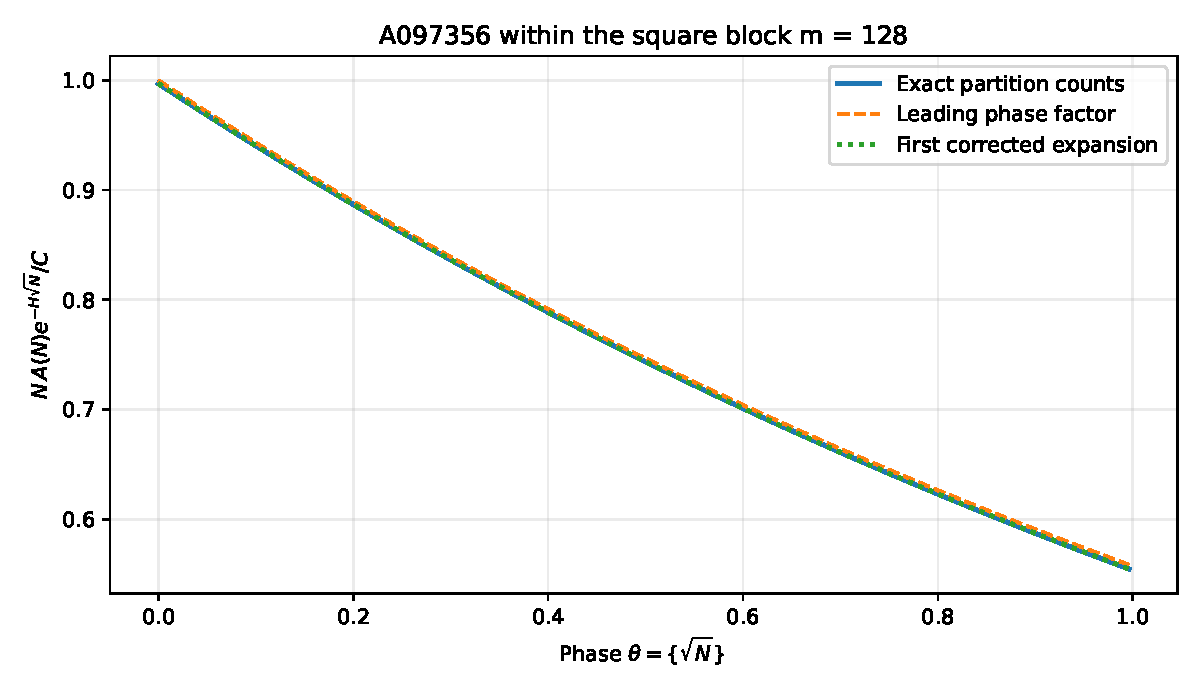
\includegraphics[width=.94\textwidth]{figures/phase_profile.pdf}
\caption{The normalized sequence within $128^2\le N<129^2$.
The exact counts and the first corrected expansion nearly coincide at
this scale. The leading phase factor varies by a fixed, nonvanishing
amount as the block is traversed.}
\label{srp:fig:phase}
\end{figure}

\subsection{Sharp envelopes and the absence of a single constant}
The leading uniform formula gives
\begin{equation}
 R(N)=C\rho^\theta(1+O(t^{-1})).
 \label{srp:eq:Rleading}
\end{equation}
Since $0<\rho<1$, every cluster value lies in $[C\rho,C]$. Squares have
$\theta=0$ and yield $C$; the integers immediately before squares have
$\theta\to1$ and yield $C\rho$. Every intermediate phase is approached
by choosing integers nearest $(m+\theta_0)^2$ for fixed
$0<\theta_0<1$. This proves the remaining parts of
\cref{srp:thm:main-phase}.

It also proves that no constant $c_0$ can satisfy
$A(N)\sim c_0d^{\sqrt N}/N$ on the whole sequence. A power-series
correction with constant coefficients cannot repair this: the missing
factor $\rho^\theta$ is of order one, not a small remainder. Finally,
\begin{equation}
 C_-=C(1-\e^{-u})=C-C\e^{-u}.
 \label{srp:eq:amplitude-difference}
\end{equation}
Thus the conjectured lower constant is the difference of the previously
recorded leading amplitudes of A206226 and A206240. This identity is a
relation among amplitudes, not an assertion of a termwise identity of
the integer sequences.

\section{Why exactly three integers fall below the lower envelope}
\label{srp:sec:threeproof}

\subsection{Strict decrease of the normalized values within each block}
\begin{lemma}
\label[lemma]{srp:lem:block-decrease}
For every sufficiently large $m$, the function
$N\mapsto R(N)$ is strictly decreasing on the integers in
$[m^2,(m+1)^2-1]$.
\end{lemma}
\begin{proof}
Write $N=m^2+\sigma m$, where $0\le\sigma\le2$. The all-orders theorem
with $K=1$ and $\tau=0$ gives, uniformly in $\sigma$,
\[
 \log p_m(N)=Hm+\sigma u-2\log m+\log C
             +\frac{D_1(\sigma,0)}m+O(m^{-2}).
\]
When $N,N+1$ stay in the same block, $\sigma$ increases by $1/m$.
Since $D_1$ is a fixed polynomial with bounded derivative on this range,
\[
 \log\frac{p_m(N+1)}{p_m(N)}=\frac um+O(m^{-2}).
\]
No differentiation of an unknown remainder is used: subtracting two
uniform $O(m^{-2})$ remainders remains $O(m^{-2})$. Also
$\log((N+1)/N)=O(m^{-2})$ and
$\sqrt{N+1}-\sqrt N=1/(2m)+O(m^{-2})$. Hence
\begin{equation}
 \log\frac{R(N+1)}{R(N)}
 =\frac{u-H/2}{m}+O(m^{-2})
 =\frac{\log\rho}{2m}+O(m^{-2})<0
 \label{srp:eq:block-ratio}
\end{equation}
for all sufficiently large $m$, uniformly within the block.
\end{proof}

\subsection{An endpoint expansion with a decisive first correction}
\begin{proposition}
\label[proposition]{srp:prop:endpoint}
For every fixed positive integer $r$, let $N_{m,r}=(m+1)^2-r$. Then
\begin{equation}
 \frac{R(N_{m,r})}{C_-}
 =1+\frac{\kappa_r}{m}+O(m^{-2}),\qquad
 \kappa_r=P_1(1)+\frac r2(H-2u).
 \label{srp:eq:kappa}
\end{equation}
In particular, $\kappa_3<0<\kappa_4$.
\end{proposition}
\begin{proof}
For fixed $r$,
\[
 t=\sqrt{(m+1)^2-r}=m+1-\frac r{2m}+O(m^{-2}),
 \qquad \theta=1-\frac r{2m}+O(m^{-2}).
\]
Use \eqref{srp:eq:main-phase} with $K=1$. The phase factor relative to its
lower limiting value is
\[
 \rho^{\theta-1}
 =1-\frac{r\log\rho}{2m}+O(m^{-2}),
\]
and $P_1(\theta)/t=P_1(1)/m+O(m^{-2})$. Their product yields
\eqref{srp:eq:kappa}. The identity $-\log\rho=H-2u$ gives its stated form.
The inequalities $\kappa_3<0<\kappa_4$ are certified by exact rational
interval arithmetic using the analytic bounds in
\cref{srp:sec:certificate}. The resulting enclosures are
\begin{align}
 -0.01618049251495
 &<\kappa_3<-0.01618049246590,\notag\\
 0.27622943999435
 &<\kappa_4<0.27622944004564.
 \label{srp:eq:kappa-certified}
\end{align}
In particular, the negative sign of $\kappa_3$ is not being inferred
from an uncertified floating-point evaluation near zero.
\end{proof}

\begin{proof}[Proof of \cref{srp:thm:three}]
By \cref{srp:prop:endpoint}, for every sufficiently large $m$, the third-last
point is strictly below $C_-$ and the fourth-last point is strictly
above $C_-$. By \cref{srp:lem:block-decrease}, all earlier points lie above
$C_-$, and all later points lie below $C_-$. This proves exactly
\eqref{srp:eq:three}.

For the upper envelope, the rational certificate gives $c<0$ and
$a+\max(b,0)<0$. Consequently $P_1(\theta)\le-\delta$ for a fixed
$\delta>0$ throughout $0\le\theta\le1$. The uniform expansion gives
\[
 R(N)=C\rho^\theta\bigl(1+P_1(\theta)/t+O(t^{-2})\bigr)<C
\]
for all sufficiently large $N$.

There are exactly three lower-envelope violations in every sufficiently
large complete block. The number of complete blocks before $X$ is
$\sqrt X+O(1)$, and the final incomplete block contributes at most three.
Finitely many initial blocks affect only the $O(1)$ constant. Thus the
violation count is $3\sqrt X+O(1)$.
\end{proof}

\paragraph{Interpretation of the OEIS conjecture.}
The sharp lower \emph{asymptotic constant} is correct. A literal eventual
inequality with that exact constant is false infinitely often, but only
at a set of natural density zero. Replacing $C_-$ by any smaller positive
constant gives an eventual lower inequality by the proved limit inferior.
No statement here asserts that Kote\v{s}ovec intended the stronger
interpretation rather than an asymptotic envelope.

\section{A limiting distribution for the normalized coefficients}
\label{srp:sec:distribution}

\begin{lemma}[Elementary phase equidistribution]
\label[lemma]{srp:lem:equidist}
Uniformly for $0\le s\le1$,
\begin{equation}
 \#\{1\le N\le M:\{\sqrt N\}\le s\}=sM+O(\sqrt M).
 \label{srp:eq:equidistribution}
\end{equation}
\end{lemma}
\begin{proof}
In a complete block $m^2\le N<(m+1)^2$, the count with phase at most $s$
is $\lfloor2ms+s^2\rfloor+1$, except for the harmless endpoint adjustment
at $s=1$. It differs from $s(2m+1)$ by $O(1)$ uniformly in $s$.
There are $O(\sqrt M)$ complete blocks, and the final incomplete block
contains $O(\sqrt M)$ indices. Sum these estimates; removing $N=0$
changes the result by at most one.
\end{proof}

\begin{theorem}[Log-uniform limiting law]
\label{srp:thm:distribution}
In empirical distribution over $1\le N\le M$, $R(N)/C$ converges to
$\rho^U$, where $U$ is uniform on $[0,1]$. Its cumulative distribution
function on $[\rho,1]$ is
\begin{equation}
 F_*(z)=1-\frac{\log z}{\log\rho},
 \qquad f_*(z)=-\frac1{z\log\rho}.
 \label{srp:eq:distribution}
\end{equation}
For every real $p\ne0$,
\begin{equation}
 \lim_{M\to\infty}\frac1M\sum_{N=1}^M R(N)^p
 =C^p\frac{\rho^p-1}{p\log\rho}.
 \label{srp:eq:moments}
\end{equation}
\end{theorem}
\begin{proof}
Equation \eqref{srp:eq:Rleading} approximates $R(N)/C$ by
$\rho^{\{\sqrt N\}}$ with error tending uniformly to zero outside a fixed
finite initial segment. Apply \cref{srp:lem:equidist} to continuous test
functions of the phase, then use uniform continuity to replace the
phase expression by the normalized coefficients. Since $\rho^U$ is a
strictly decreasing continuous transformation of $U$, its distribution
function is as displayed. Integrating $C^p\rho^{ps}$ over $0\le s\le1$
gives \eqref{srp:eq:moments}. Negative moments are allowed because the
normalized sequence stays bounded away from zero for large $N$; the
finitely many initial positive terms have vanishing empirical weight.
\end{proof}

The description as a distribution does not posit a random model for
$A(N)$. It describes deterministic frequencies of its normalized values.
The three lower-envelope exceptions per large block are compatible with
this law: they have density zero and approach its lower endpoint.

\writenotefour{The lemma and theorem below come from manuscript~02 of
batch~74 (\cref{srp:se:sec:second}). They add a rate to
\cref{srp:thm:distribution} for Lipschitz test functions. Write
$\beta=-\log\rho=H-2u$.}

\begin{lemma}[Phase equidistribution with a rate; manuscript~02]
\label[lemma]{srp:se:lem:equidist}
For every Lipschitz function $f:[0,1]\to\R$,
\begin{equation}
 \frac1M\sum_{N=1}^Mf(\{\sqrt N\})=\int_0^1f(x)\dd x+O_f(M^{-1/2}).
 \label{srp:se:eq:equidist}
\end{equation}
\end{lemma}
\begin{proof}[Proof (manuscript~02)]
On a complete block $k^2\le N<(k+1)^2$, comparing a Riemann sum with its
integral gives
$\sum_{N=k^2}^{(k+1)^2-1}f(\sqrt N-k)=\int_0^1f(x)\,2(k+x)\dd x+O_f(1)$,
because $f(\sqrt y-k)$ varies by $O_f(k^{-1})$ across each of the $2k+1$
unit intervals. Summing the blocks $k<K$ gives
$K^2\int_0^1f+O_f(K)$, since the bounded part $2x$ of the weight changes
each block sum by $O_f(1)$. The final incomplete block has
$O(\sqrt M)$ terms. Divide by $M$.
\end{proof}

As this write adds, the lemma also follows from \cref{srp:lem:equidist}:
writing the average as
a Stieltjes integral of $f$ against the empirical distribution function of
the phases and integrating by parts, the discrepancy $O(M^{-1/2})$ of
\eqref{srp:eq:equidistribution} becomes an error $O(\operatorname{Lip}(f)M^{-1/2})$.

\begin{theorem}[Rate in the log-uniform law; manuscript~02]
\label{srp:se:thm:law}
For every Lipschitz function $\varphi$ on a compact interval containing
$[C_-,C]$ and all the values $R(N)$, $N\ge1$,
\begin{equation}
 \frac1M\sum_{N=1}^M\varphi(R(N))
 =\frac1\beta\int_{C_-}^{C}\frac{\varphi(r)}r\dd r+O_\varphi(M^{-1/2}).
 \label{srp:se:eq:law}
\end{equation}
Changing finitely many initial terms does not affect the statement. The
limiting density is $1/(\beta r)$ on $[C_-,C]$, the distribution of
\eqref{srp:eq:distribution}, and
\begin{equation}
 \lim_{M\to\infty}\frac1M\sum_{N=1}^M\log R(N)=\log C-\frac\beta2.
 \label{srp:se:eq:logmean}
\end{equation}
\end{theorem}
\begin{proof}[Proof (manuscript~02)]
By \eqref{srp:eq:Rleading}, $R(N)-C\rho^{\{\sqrt N\}}=O(N^{-1/2})$ for large
$N$. The average change of a Lipschitz test function is therefore at most a
constant times $M^{-1}\sum_{N\le M}N^{-1/2}=O(M^{-1/2})$, the finitely many
initial terms contributing $O(M^{-1})$. Apply \cref{srp:se:lem:equidist}
to $f(x)=\varphi(C\rho^x)$ and substitute $r=C\rho^x$,
$\dd x=-\dd r/(\beta r)$. For \eqref{srp:se:eq:logmean} take
$\varphi=\log$, Lipschitz on a compact interval of positive reals that
contains every $R(N)$ (all are positive, and they converge to
$[C_-,C]$), and integrate.
\end{proof}

Manuscript~02 also derives the moments \eqref{srp:eq:moments}, in the form
$C^q(1-\rho^q)/(q\beta)$. Neither the arithmetic nor the geometric mean of
$R(N)$ is the upper or lower limiting constant. The theorem bears on the
question about an effective error term in \cref{srp:sec:future}; see the
note there.

\section{Summation across square blocks}
\label{srp:sec:summation}

The unsmoothed coefficients jump at squares because the allowed part
size increases. Their partial sums have a different phase law.

\begin{theorem}[Summatory asymptotic]
\label{srp:thm:sum}
Let $S(N)=\sum_{n=0}^N A(n)$, $m=\lfloor\sqrt N\rfloor$, and
$\theta=\sqrt N-m$. Then uniformly in $\theta\in[0,1)$,
\begin{equation}
 S(N)=\frac{C\e^{Hm}}{u m}
 \left(\e^{2u\theta}-1+
       \frac{\e^{2u}-1}{\e^H-1}\right)
 \left(1+O(m^{-1})\right).
 \label{srp:eq:sum}
\end{equation}
\end{theorem}
\begin{proof}
In block $m$, the leading bounded-offset formula is
\[
 A(m^2+j)=\frac{C\e^{Hm}}{m^2}\e^{uj/m}(1+O(m^{-1})),
 \qquad 0\le j\le2m,
\]
uniformly in $j$. With $J=N-m^2=2m\theta+\theta^2$, summing the geometric
progression through $j=J$ gives
\begin{equation}
 \sum_{j=0}^{J}A(m^2+j)
 =\frac{C\e^{Hm}}{u m}(\e^{2u\theta}-1)
   +O(\e^{Hm}/m^2).
 \label{srp:eq:partial-block}
\end{equation}
This is an additive error estimate, valid even when $\theta=0$ and its
displayed leading term vanishes. A complete earlier block $k$ contributes
\[
 \frac{C\e^{Hk}}{u k}(\e^{2u}-1)
 +O(\e^{Hk}/k^2).
\]
For $m/2\le k=m-l<m$, replace $m/k$ by $1+O(l/m)$ and use the convergent
sums $\sum_{l\ge1}\e^{-Hl}$ and $\sum_{l\ge1}l\e^{-Hl}$. This yields
\[
 \sum_{k<m}\sum_{n=k^2}^{(k+1)^2-1}A(n)
 =\frac{C\e^{Hm}}{u m}\frac{\e^{2u}-1}{\e^H-1}
  +O(\e^{Hm}/m^2).
\]
The blocks $k<m/2$ are exponentially smaller: the same leading bound
controls all sufficiently large such $k$, and the remaining finite
initial segment is negligible. This justifies the summation without an
uncontrolled interchange of a nonuniform asymptotic series.

Add \eqref{srp:eq:partial-block}. The bracket in \eqref{srp:eq:sum} is bounded
below by the positive constant $(\e^{2u}-1)/(\e^H-1)$, so the additive
error may be written as the stated relative error uniformly.
\end{proof}

The leading expression glues continuously across a square. If
$B=(\e^{2u}-1)/(\e^H-1)$, then
$\e^{2u}-1+B=\e^H B$. Thus the limiting value at the end of one block
matches the next block's leading value, after the common change in its
$\e^{Hm}$ scale. This is a useful example of summation removing a jump
while retaining a nonconstant phase profile.

\section{Inverting the square subsequence}
\label{srp:sec:square-inverse}

First remove the floor phase by considering $b(m)=p_m(m^2)$.
Write $D_j=D_j(0,0)$ and define its logarithmic coefficients by
\begin{equation}
 \log\left(1+\sum_{j\ge1}D_j z^j\right)=\sum_{j\ge1}L_j z^j.
 \label{srp:eq:Ldef}
\end{equation}
A finite recurrence is
\begin{equation}
 L_n=D_n-\frac1n\sum_{j=1}^{n-1}jL_jD_{n-j}.
 \label{srp:eq:Lrec}
\end{equation}
For example $L_1=D_1$, $L_2=D_2-D_1^2/2$, and
$L_3=D_3-D_1D_2+D_1^3/3$.

\subsection{The Lambert core and formal reversion}
The dominant real equation is
\begin{equation}
 \frac{C\e^{HX}}{X^2}=Y,
 \qquad HX-2\log X=\log Y-\log C.
 \label{srp:eq:core-equation}
\end{equation}
For $X>2/H$ it is strictly increasing and has the inverse
\eqref{srp:eq:core}, using $W_{-1}$, not $W_0$. The principal branch would
select the small solution of the same algebraic rearrangement and is
not the desired asymptotic inverse.

\begin{proposition}[All-orders inverse coefficients]
\label[proposition]{srp:prop:inverse-coeff}
The formal inverse of the square-subsequence expansion has the unique
form
\begin{equation}
 \widehat x(Y)=X(Y)+\sum_{r\ge1}q_rX(Y)^{-r}.
 \label{srp:eq:inverse-series}
\end{equation}
If $\Delta_{r-1}(X)=\sum_{j=1}^{r-1}q_jX^{-j}$, then
\begin{equation}
 q_r=-\frac1H[X^{-r}]
 \left\{-2\log\left(1+\frac{\Delta_{r-1}}X\right)
 +\sum_{j=1}^r L_j(X+\Delta_{r-1})^{-j}\right\}.
 \label{srp:eq:qrec}
\end{equation}
In particular,
\begin{align}
 q_1&=-L_1/H,\notag\\
 q_2&=-2L_1/H^2-L_2/H,\notag\\
 q_3&=(2q_2+L_1q_1-L_3)/H.
 \label{srp:eq:qfirst}
\end{align}
\end{proposition}
\begin{proof}
Put $x=X+\Delta$ in
$Hx-2\log x+\sum_{j\ge1}L_jx^{-j}=\log Y-\log C$ and subtract
\eqref{srp:eq:core-equation}. The resulting equation is
\[
 H\Delta-2\log(1+\Delta/X)+\sum_{j\ge1}L_j(X+\Delta)^{-j}=0.
\]
At order $X^{-r}$ the previously unknown coefficient occurs only as
$Hq_r$, since all its occurrences in the logarithm and inverse powers
carry at least one additional negative power of $X$. This proves both
uniqueness and the recurrence. Equating the first three coefficients
gives \eqref{srp:eq:qfirst}.
\end{proof}

Numerically the first coefficients are
\begin{align*}
 q_1&=0.169152574435079450236784971776\ldots,\\
 q_2&=0.151490069409063238951250698423\ldots,\\
 q_3&=0.108853991540605915550641858907\ldots,\\
 q_4&=0.058606290184968379522730931714\ldots.
\end{align*}
To express the same expansion using only iterated logarithms, put
$\Lambda=\log(Y/(CH^2))$. Reversion of
$HX-2\log(HX)=\Lambda$ and inclusion of the first correction give
\begin{equation}
 \widehat x(Y)=\frac1H\left(
 \Lambda+2\log\Lambda+
 \frac{4\log\Lambda-HL_1}{\Lambda}
 +O\left(\frac{(\log\Lambda)^2}{\Lambda^2}\right)\right).
 \label{srp:eq:log-inverse}
\end{equation}
The Lambert form keeps the entire leading power--logarithmic core
unexpanded and is usually more accurate at a given truncation order.

\subsection{What a real inverse means for an integer sequence}
The integer data $b(m)$ do not specify a canonical smooth interpolation.
To state a rigorous analytic meaning without inventing one, fix $K$ and
use the explicit smooth approximation
\begin{equation}
 B_K(x)=\frac{C\e^{Hx}}{x^2}
 \left(1+\sum_{j=1}^K D_jx^{-j}\right).
 \label{srp:eq:BK}
\end{equation}
It is positive and strictly increasing for sufficiently large $x$, since
$(\log B_K)'(x)=H-2/x+O(x^{-2})$. Let $x_K(Y)$ denote its unique large
inverse. The formal calculation and the mean value theorem show
\begin{equation}
 x_K(Y)=X(Y)+\sum_{j=1}^K q_jX(Y)^{-j}+O(X(Y)^{-K-1}).
 \label{srp:eq:real-inverse}
\end{equation}
Indeed substitution of the right-hand truncation leaves a logarithmic
residual of order $X^{-K-1}$, and the derivative of the logarithmic
left-hand side is bounded away from zero near the root.

\begin{proposition}[Transport to a discrete threshold]
\label[proposition]{srp:prop:ceil}
Let $M(Y)=\min\{m\ge0:b(m)\ge Y\}$. There is a constant $c_K>0$ such that,
for all sufficiently large $Y$, with
$\delta_K=c_Kx_K(Y)^{-K-1}$,
\begin{equation}
 \ceil{x_K(Y)-\delta_K}\ \le M(Y)\le\
 \ceil{x_K(Y)+\delta_K}.
 \label{srp:eq:ceil-brackets}
\end{equation}
The same type of brackets holds with $x_K$ replaced by the explicit
truncation in \eqref{srp:eq:real-inverse}, after enlarging $c_K$.
\end{proposition}
\begin{proof}
At integer $m$, \cref{srp:thm:allorders} gives
$\log b(m)-\log B_K(m)=O(m^{-K-1})$. Near $x_K$, the logarithmic
derivative of $B_K$ is at least $H/2$ for large $Y$. Displacing the
argument by a sufficiently large constant times $x_K^{-K-1}$ therefore
makes the sign of $\log b(m)-\log Y$ certain on either side of the
bracket. Monotonicity of $b(m)$ excludes more distant threshold values.
Taking ceilings yields \eqref{srp:eq:ceil-brackets}. The real approximation
error \eqref{srp:eq:real-inverse} has the same order and can be absorbed by
increasing the constant.
\end{proof}

A ceiling cannot in general be pulled through an $O(\cdot)$ term.
An exact formula $M(Y)=\lceil x_K(Y)\rceil$ follows from
\eqref{srp:eq:ceil-brackets} only under a separation condition that ensures
both endpoint ceilings agree, for example
$\dist(x_K(Y),\mathbb Z)>\delta_K$. Arbitrarily small real errors can
change a ceiling near an integer. This is the reason to keep the real
inverse and the staircase statement distinct, as in ProveIt's
remainder-transport and staircase organization \cite{proveit}.

\writenote{\Cref{srp:prop:ceil} and the separation remark after it are
not new. They are the special case $x_\ast=x_K(Y)$, $\eta=\delta_K$ of
the staircase recovery theorem of ProveIt's transseries volume
\cite{proveitTI}, Theorem \texttt{p0:thm:staircase}. Once the real
inverse $\nu$ of a strictly increasing interpolation of $b$ is known to
lie within $\delta_K$ of $x_K(Y)$, its part~(1), exact rounding
$M(Y)=\lceil\nu(Y)\rceil$, and the monotonicity of the ceiling give the
bracket \eqref{srp:eq:ceil-brackets}, and its part~(2), the separation
condition $\lceil x_\ast-\eta\rceil=\lceil x_\ast+\eta\rceil$, gives the
exact formula $M(Y)=\lceil x_K(Y)\rceil$. The order-theoretic content of
part~(2) is formalized in Lean as \texttt{Fabius.staircase\_separation}
(with \texttt{Fabius.staircase\_ceil} for part~(1)) in
\nolinkurl{Analysis/FabiusFunction/Lean/FabiusFunction/StaircaseInversion.lean}
\cite{proveitLean}. What is specific to A097356 here is the analytic
input: the all-orders estimate $\log b(m)-\log B_K(m)=O(m^{-K-1})$ of
\cref{srp:thm:allorders} that produces the width $\delta_K$. That input
is not formalized, and this report gains no formal status from the Lean
file. The proposition is printed with its delivered proof as a
specialization, not as a new result.}

For $p_m(m^2+sm)$ with $s=\pm1$, replace $C$ by $C\e^{su}$ and $D_j$ by
$D_j(s,0)$. All the same reversion and threshold arguments apply.

\section{Inverting the complete floor-dependent sequence}
\label{srp:sec:full-inverse}

\subsection{Monotonicity and the geometry of a square block}
The sequence $A(N)$ is nondecreasing: append a part of size one to a
partition counted at $N$; the resulting partition is allowed at $N+1$
because the cutoff cannot decrease. The map is injective. Since
$A(m^2)\sim Cd^m/m^2\to\infty$, the inverse threshold $Q(Y)$ is finite.

For a real phase $s\in[0,1)$ and integer points with $\sqrt N=m+s$, the
leading logarithm is
\begin{equation}
 \log A(N)=\log C+Hm+2us-2\log m+O(m^{-1}).
 \label{srp:eq:log-block}
\end{equation}
As a block is traversed, this logarithm increases by about $2u$; at the
next square, the leading jump is $H-2u=-\log\rho>0$. Thus a positive
fraction of large target logarithms lie in gaps crossed at a single
square. A smooth phase-blind inverse cannot see these plateaus.

\subsection{Proof of the global inverse approximation}
\begin{proof}[Proof of \cref{srp:thm:main-inverse}]
The core $X=X(Y)$ satisfies
$\log Y=\log C+HX-2\log X$. Uniform bounds on the phase factor in
\eqref{srp:eq:main-phase} first imply
\begin{equation}
 \sqrt{Q(Y)}=X+O(1).
 \label{srp:eq:coarse-inverse}
\end{equation}
For example, changing $t$ by a sufficiently large fixed constant changes
$Ht-2\log t$ by more than the bounded phase correction, and comparison
with the nearest available integer index brackets the threshold.

It is therefore enough to consider $t=X+O(1)$, where
$\log\lfloor t\rfloor=\log X+O(X^{-1})$. Define the right-continuous
increasing comparison function
\begin{equation}
 g_X(t)=\log C-2\log X+H\lfloor t\rfloor
        +2u\{t\}.
 \label{srp:eq:gX}
\end{equation}
At the available grid points $t=\sqrt N$ near $X$,
\eqref{srp:eq:log-block} gives
$\log A(N)=g_X(t)+O(X^{-1})$, uniformly. The generalized real inverse
of $g_X$ at $\log Y$ is exactly $T(X)$: if $X=k+\eta$, then the target
increment in block $k$ is $H\eta$; it is attained at phase
$\eta/\gamma$ when $\eta\le\gamma$, and otherwise the first crossing is
at $k+1$.

The map $T$ is continuous and nondecreasing, with slopes $1/\gamma$
and $0$ on its linear pieces. The generalized inverse of $g_X$ is
therefore globally Lipschitz as a function of the target logarithm,
with constant $1/(2u)$. A perturbation of that logarithm by
$O(X^{-1})$ displaces its inverse by $O(X^{-1})$, even at the beginning
or end of a plateau. The grid spacing
$\sqrt{N+1}-\sqrt N$ near $X$ is also $O(X^{-1})$. Comparing the target
with $g_X\pm c/X$ and then moving to the neighboring grid points proves
\[
 \sqrt{Q(Y)}=T(X)+O(X^{-1}).
\]
Since $T(X)=X+O(1)$, squaring changes the error to $O(1)$, as stated.
\end{proof}

Write
\begin{equation}
 \psi(\eta)=\min(\eta/\gamma,1)-\eta
 =\begin{cases}
 (1/\gamma-1)\eta,&0\le\eta\le\gamma,\\
 1-\eta,&\gamma\le\eta\le1.
 \end{cases}
 \label{srp:eq:tent}
\end{equation}
Then $T(X)=X+\psi(\{X\})$, and the global inverse theorem gives
\begin{equation}
 Q(Y)-X(Y)^2=2X(Y)\psi(\{X(Y)\})+O(1).
 \label{srp:eq:inverse-missing-term}
\end{equation}
For a fixed phase $\eta_0\in(0,1)$, set
$Y_k=C\e^{H(k+\eta_0)}/(k+\eta_0)^2$. Then $X(Y_k)=k+\eta_0$ and
$\psi(\eta_0)>0$. Along these targets the omitted term has size
$\Theta(X)$. Rounding $Y_k$ to a nearby integer changes $X$ by an
exponentially small amount and does not alter this conclusion. The
phase-blind error is thus genuinely of order $\log Y$, not just a loose
upper bound or a one-integer rounding issue.

\begin{figure}[htbp]
\centering
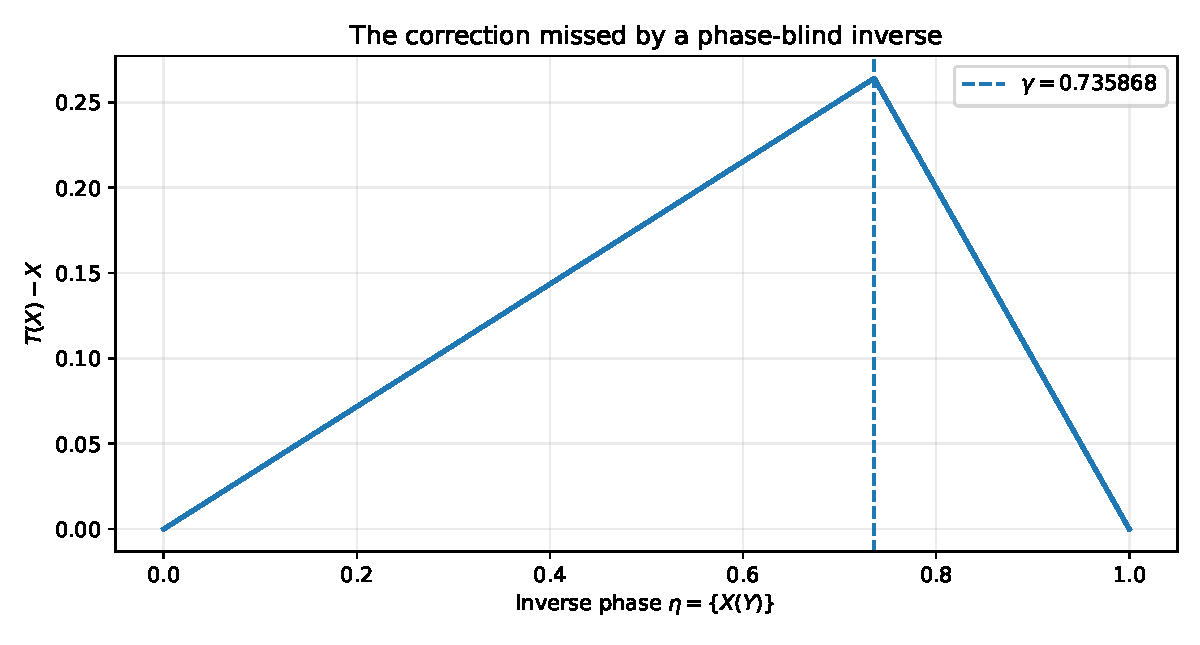
\includegraphics[width=.94\textwidth]{figures/inverse_phase.pdf}
\caption{The tent-shaped correction $\psi(\eta)=T(X)-X$. Its maximum is
$1-\gamma=0.264131709289\ldots$. The flat pieces of $T$, not of $\psi$,
correspond to target ranges whose inverse is the next perfect square.}
\label{srp:fig:inverse}
\end{figure}

\subsection{Exact plateaus away from the transition layers}
\begin{proposition}
\label[proposition]{srp:prop:plateaus}
Fix a compact interval $J\subset(\gamma,1)$. If $X(Y)=k+\eta$ with
$\eta\in J$, then for all sufficiently large $k$,
\begin{equation}
 Q(Y)=(k+1)^2.
 \label{srp:eq:plateaus}
\end{equation}
\end{proposition}
\begin{proof}
At the last index of block $k$,
\[
 \log A((k+1)^2-1)=\log C+Hk+2u-2\log k+O(k^{-1}).
\]
At the next square,
\[
 \log A((k+1)^2)=\log C+H(k+1)-2\log(k+1)+O(k^{-1}).
\]
The target logarithm is
$\log C+Hk+H\eta-2\log k+O(k^{-1})$. On $J$, both
$H\eta-2u$ and $H(1-\eta)$ have positive lower bounds. Thus the target
lies strictly between these two adjacent values for large $k$.
Monotonicity proves the result.
\end{proof}

\subsection{The first interior correction}
Fix instead a compact interval $J\subset(0,\gamma)$. Let $X=k+\eta$ with
$\eta\in J$, and put
\begin{equation}
 \sigma_0(\eta)=\frac{H\eta}{u},\qquad
 \tau_0(\eta)=\frac{-2\eta-D_1(\sigma_0(\eta),0)}{u}.
 \label{srp:eq:interior-coeff}
\end{equation}
Consider the real approximation
\begin{equation}
 n_*(Y)=k^2+\sigma_0(\eta)k+\tau_0(\eta).
 \label{srp:eq:interior-root}
\end{equation}
It is useful for locating the integer threshold even though no canonical
interpolation of $A(N)$ is being specified.

\begin{proposition}[Interior threshold brackets]
\label[proposition]{srp:prop:interior}
Uniformly for $\eta\in J$, there is a constant $c_J>0$ such that for all
sufficiently large $k$,
\begin{equation}
 \ceil{n_*(Y)-c_J/k}\le Q(Y)\le\ceil{n_*(Y)+c_J/k}.
 \label{srp:eq:interior-bracket}
\end{equation}
In particular $Q(Y)=\lceil n_*(Y)\rceil$ whenever the endpoint ceilings
in \eqref{srp:eq:interior-bracket} agree.
\end{proposition}
\begin{proof}
For $N=k^2+\sigma_0k+\tau$,
\cref{srp:thm:allorders} gives
\[
 \log p_k(N)=\log C+Hk-2\log k+u\sigma_0
 +\frac{u\tau+D_1(\sigma_0,0)}k+O(k^{-2}).
\]
The target has expansion
\[
 \log Y=\log C+Hk-2\log k+H\eta-\frac{2\eta}{k}
 +O(k^{-2}).
\]
Matching its constant and $k^{-1}$ terms gives
\eqref{srp:eq:interior-coeff}. The slope of the logarithmic asymptotic
approximation with respect to $N$ is $u/k+O(k^{-2})>0$. Hence a
logarithmic residual $O(k^{-2})$ gives a real index displacement
$O(k^{-1})$. Equivalently, evaluating at integer points a sufficiently
large constant times $1/k$ on either side of $n_*$ makes the signs
certain. The compact separation from $0$ and $\gamma$ keeps these points
in block $k$ and away from its jumps. Monotonicity and ceilings yield
\eqref{srp:eq:interior-bracket}.
\end{proof}

\subsection{An all-orders interior recurrence}
Let
\begin{equation}
 \log\left(1+\sum_{j\ge1}D_j(\sigma,0)w^j\right)
 =\sum_{j\ge1}L_j(\sigma)w^j.
 \label{srp:eq:Lj-sigma}
\end{equation}
Every $L_j(\sigma)$ is a polynomial obtained from
\eqref{srp:eq:Lrec}. Define a formal series
$\sigma(w,\eta)=\sum_{r\ge0}\sigma_r(\eta)w^r$, beginning with
$\sigma_0=H\eta/u$. The equation to be solved is
\begin{equation}
 u\sigma(w,\eta)+\sum_{j\ge1}L_j(\sigma(w,\eta))w^j
 =H\eta-2\log(1+\eta w).
 \label{srp:eq:interior-equation}
\end{equation}
If $\sigma^{<r}(w,\eta)=\sum_{v=0}^{r-1}\sigma_v(\eta)w^v$, the next
coefficient is explicitly
\begin{equation}
 \sigma_r(\eta)=\frac1u\left\{
 \frac{2(-1)^r\eta^r}{r}
 -[w^r]\sum_{j=1}^r L_j(\sigma^{<r}(w,\eta))w^j
 \right\},\qquad r\ge1.
 \label{srp:eq:interior-recurrence}
\end{equation}
The unknown $\sigma_r$ occurs only through $u\sigma_r$ at order $w^r$;
this proves formal uniqueness. At $r=1$ it gives precisely $\tau_0$.
For a truncation through $r=R$ put
\[
 n_R(Y)=k^2+k\sum_{r=0}^R\sigma_r(\eta)k^{-r}.
\]
The analytic remainder argument used in \cref{srp:prop:interior}, now with
\cref{srp:thm:allorders} at higher order, yields uniform brackets
\begin{equation}
 \ceil{n_R(Y)-c_{J,R}k^{-R}}
 \le Q(Y)\le
 \ceil{n_R(Y)+c_{J,R}k^{-R}}.
 \label{srp:eq:interior-allorders}
\end{equation}
Indeed the logarithmic residual is $O(k^{-R-1})$ and the local logarithmic
slope is comparable to $1/k$. This proves an all-orders inverse
expansion on every compact interior phase interval.

No all-orders assertion is made here uniformly through $\eta=0$ or
$\eta=\gamma$. Those switching layers require their own scaled
coordinates. The coarse global formula \eqref{srp:eq:global-inverse}
\emph{does} remain uniform through both transitions.

\section{Exact and high-precision computational checks}
\label{srp:sec:numerics}

\subsection{What was computed}
The included run used Python with \texttt{mpmath} 1.3.0 at 80 decimal
digits. The counts themselves were not computed by floating point.
They were generated by the exact recurrence that adds the allowed parts
one at a time:
\begin{equation}
 p_m(N)=p_{m-1}(N)+p_m(N-m),
 \label{srp:eq:DP}
\end{equation}
with $p_0(0)=1$, $p_0(N)=0$ for $N>0$, and zero values at negative
arguments. In-place updates run over increasing $N$ for each new $m$.
The final run produced all A097356 values through $N=66048$ and the
three quadratic subsequences through $m=256$.

As transcription checks, the first 54 terms of A097356 and first 17
terms of A206226 were compared with the inspected OEIS entries
\cite{oeisA,oeisSquare}. All agreed. All 66048 consecutive monotonicity
comparisons passed. The coefficient generator was independently checked
against the closed formula \eqref{srp:eq:D1} at nine choices of $\sigma$.
The exact rational checks described in \cref{srp:sec:certificate} also
passed. These are finite checks of the supplied implementation and
specific signs; they do not replace the all-orders analytic proof.

\subsection{Square-subsequence accuracy}
\Cref{srp:tab:errors} records relative errors
$(\text{approximation}/p_m(m^2))-1$ using the truncation through $D_K$.
The rapid improvement is consistent with the successive proved powers
of $1/m$.
\begin{table}[htbp]
\centering\small
\begin{tabular}{r r r r r r}
\toprule
$m$ & $K=0$ & $K=1$ & $K=2$ & $K=3$ & $K=4$\\
\midrule
16  & $2.37\,10^{-2}$ & $-2.89\,10^{-4}$ & $2.71\,10^{-6}$ & $-9.65\,10^{-8}$ & $-1.65\,10^{-8}$\\
32  & $1.18\,10^{-2}$ & $-7.18\,10^{-5}$ & $3.42\,10^{-7}$ & $-4.88\,10^{-9}$ & $5.60\,10^{-11}$\\
64  & $5.87\,10^{-3}$ & $-1.79\,10^{-5}$ & $4.28\,10^{-8}$ & $-3.05\,10^{-10}$ & $1.74\,10^{-12}$\\
128 & $2.93\,10^{-3}$ & $-4.46\,10^{-6}$ & $5.35\,10^{-9}$ & $-1.91\,10^{-11}$ & $5.42\,10^{-14}$\\
256 & $1.46\,10^{-3}$ & $-1.12\,10^{-6}$ & $6.69\,10^{-10}$ & $-1.19\,10^{-12}$ & $1.69\,10^{-15}$\\
\bottomrule
\end{tabular}
\caption{Relative errors for A206226. The CSV files retain more digits.
Here $a\,10^{-j}$ means $a\times10^{-j}$.}
\label{srp:tab:errors}
\end{table}

A single small-$m$ accuracy pattern does not prove convergence of the
asymptotic series or identify secondary saddles. For example, the
$m=16$ row need not follow the eventual algebraic error ratios as cleanly
as the larger rows. No inference about exponentially small sectors is
based on that observation.

\subsection{The third-last point is a subtle case}
The table below shows
$R((m+1)^2-r)/C_- -1$ near the end of a block.
\begin{table}[htbp]
\centering\small
\begin{tabular}{r r r r r}
\toprule
$m$ & $r=1$ & $r=2$ & $r=3$ & $r=4$\\
\midrule
16 & $-0.03435127$ & $-0.01580701$ & $0.003070873$ & $0.02228763$\\
32 & $-0.01793700$ & $-0.008717003$ & $0.000586331$ & $0.009973718$\\
64 & $-0.009173963$ & $-0.004582366$ & $0.0000300765$ & $0.004663456$\\
128 & $-0.004640419$ & $-0.002350006$ & $-0.0000543790$ & $0.002246474$\\
256 & $-0.002333841$ & $-0.001190087$ & $-0.0000450293$ & $0.001101334$\\
\bottomrule
\end{tabular}
\caption{The third-last index changes sign later than the last two.
The eventual theorem rests on the certified $\kappa_3<0$, not on
extrapolation from these samples.}
\label{srp:tab:endpoints}
\end{table}

The four limiting coefficients in \eqref{srp:eq:kappa} are approximately
\[
 (\kappa_1,\kappa_2,\kappa_3,\kappa_4)
 =(-0.60100036,-0.30859043,-0.01618049,0.27622944).
\]
In particular, the small absolute size of $\kappa_3$ explains why an
initial data inspection could miss the eventual third exception.

\subsection{Inverse accuracy and the plateaus}
For the inverse tests, target values were chosen as integers near
$C\e^{H(k+\eta)}/(k+\eta)^2$; thresholds were then found by binary search
in the exact integer table. \Cref{srp:tab:inverse-errors} gives the block
$k=128$ results. ``Interior ceiling'' means the value
$\lceil n_*(Y)\rceil$ from \eqref{srp:eq:interior-root}; it is only used on
interior phases.
\begin{table}[htbp]
\centering\small
\begin{tabular}{r r r r r}
\toprule
$\eta$ & Exact $Q(Y)$ & $X^2-Q(Y)$ & $T(X)^2-Q(Y)$ & Interior ceiling error\\
\midrule
0.10 & 16420 & $-10.3900$ & $-1.1927$ & 0\\
0.30 & 16490 & $-29.1100$ & $-1.4673$ & 0\\
0.50 & 16560 & $-47.7500$ & $-1.5942$ & 0\\
0.70 & 16631 & $-67.3100$ & $-2.5733$ & 0\\
0.80 & 16641 & $-51.5600$ & $0$ & plateau\\
0.95 & 16641 & $-12.8975$ & $0$ & plateau\\
\bottomrule
\end{tabular}
\caption{An ordinary smooth inverse misses dozens of indices; the
phase map has a bounded error, and the first interior correction locates
the exact integer thresholds in these tests. Exact rounding in arbitrary
cases still requires the separation condition in the theorem.}
\label{srp:tab:inverse-errors}
\end{table}

\subsection{Reproduction and interpretation of the outputs}
From the directory containing the scripts, run
\begin{lstlisting}
python certificate.py
python verify.py --max-m 256 --output results
\end{lstlisting}
The first command uses only the Python standard library and performs
exact rational interval computations. The second needs \texttt{mpmath}
and reruns the coefficient evaluation and integer checks. Its time cost
is dominated by $O(m_{\max}^3)$ arbitrary-precision integer additions;
storage is $O(m_{\max}^2)$ integers. These are operation counts, not
constant-time bit-complexity bounds.

The data directory contains coefficient JSON files and separate CSV
files for quadratic expansions, floor expansions, endpoint values,
the last-four classification, inverse thresholds, and summatory
approximations. \texttt{verification\_summary.json} records the completed
run. The figures use a saved subset of the exact-count comparison data;
they are illustrations, not substitutes for the numerical tables or
proofs.

\writenote{In the collection the four scripts are in \texttt{code/}, and
the eleven files of the delivered \texttt{results/} directory, with the
two requirements files, are in \texttt{data/}. Run the commands above
from a copy of \texttt{code/} with an explicit output directory, for
example \texttt{--output} pointing to a scratch directory, never to the
shipped \texttt{data/}. The script writes its CSV files with CRLF line
ends on every platform, as delivered, and on Windows also writes its
JSON files with CRLF ends, so a rerun there differs from the shipped
JSON files in line ends only. The figure script reads
\texttt{results/plot\_data.json} and writes \texttt{figures/} relative
to the working directory by default; pass \texttt{--data} and
\texttt{--output} explicitly. At intake both commands were rerun on a
copy: of the ten files the driver writes, the six CSV files and
\texttt{plot\_data.json} were byte-identical to the delivery and the
other three JSON files equal apart from line ends; its standard output
equals the shipped \texttt{data/run\_log.txt}, which is a capture of
that output and not a file the script writes.}

\section{Further research questions and a formalization route}
\label{srp:sec:future}

The results suggest several nontrivial continuations. The following are
proposals, not claims that their conclusions have been proved here.

\subsection{Effective determination of the first stable three-exception block}
The analytic proof gives a finite but unspecified $m_0$. An effective
version would bound the $m^{-2}$ remainder in the endpoint formula and
in the block-ratio estimate, then combine it with certified computation
for the finite initial range. The small margin
$|\kappa_3|\approx0.01618$ makes a crude uniform bound potentially
inefficient. A useful target is the \emph{least} $m_0$ such that exactly
three exceptions occur in every block $m\ge m_0$, together with a proof
that no later reversals occur. Uncertified testing of a large interval
would not settle the latter requirement.

\writenotefour{Manuscript~02 of batch~74 records the third-last point
below the envelope in the blocks $m=79$, $99$ and $139$
(\texttt{data/02-sharp-boundary\_defects.csv}; it labels them by the upper
squares $k=80,100,140$), consistent with \cref{srp:tab:endpoints}
($m=64$ above, $m=128$ below). A computation made for this write (exact
counts by \eqref{srp:eq:DP}; the comparison with $C_-d^{\sqrt N}/N$ in
50-digit arithmetic, not interval-certified; not shipped) narrows this
further: for $60\le m\le71$ exactly the last two indices of the block are
below the envelope, and for every $72\le m\le200$ exactly the last three.
At $m=71$ and $m=72$ the third-last point lies at relative distance
$+2.8\cdot10^{-6}$ and $-3.0\cdot10^{-7}$ from it. So $m_0=72$ is the
least value compatible with these data. Proving that no reversal occurs
after $m=200$, the second half of the question, is untouched, and nothing
here is certified.}

\subsection{All-orders switching layers for the inverse}
The global inverse error is bounded, and the interior inverse has all
orders, but the transition regions have only been covered at coarse
order. Resolve the layers
$\eta=O(1/k)$ and $\eta-\gamma=O(1/k)$ by comparing corrected block
endpoints and square values. A complete formulation should give the
shifted jump thresholds, integer ceiling brackets, and a uniform
matching rule between interior roots and exact plateaus. This would
extend the phase-sensitive inverse from an atlas with excluded
transition layers to a uniformly corrected global description.

\subsection{Exponential sectors and optimal truncation}
The minor-arc proof only shows contributions smaller than every fixed
algebraic order. It does not identify their leading exponential scales.
A genuinely exponentially improved expansion should identify the
relevant rational-angle or complex saddles, compare their actions, and
describe any changes of dominance. One should also study the growth of
$D_k$ as $k\to\infty$, whether a Gevrey bound holds, and how optimal
truncation relates to the first omitted saddle. Calling the present
Poincar\'e series a complete resurgent transseries would skip these
unresolved steps.

\subsection{Other moving cutoffs and their endpoint defect counts}
For $A_c(N)=p_{\lfloor c\sqrt N\rfloor}(N)$ with fixed $c>0$, the saddle
has $\alpha=c^{-2}$. The current uniform theorem supplies the analytic
input for a related phase calculus, but the arithmetic block endpoints
need not be integer squares. Determine whether the number of points
violating a sharp asymptotic lower envelope stabilizes, becomes
periodic, or has a phase-dependent distribution. The sign of a first
endpoint correction can change with $c$, producing transitions in that
count. Rational and irrational $c^2$ may lead to genuinely different
endpoint arithmetic.

\subsection{Two simultaneous restrictions}
Partitions constrained both in largest part and number of parts are
encoded by Gaussian binomial coefficients. Jiang and Wang provide a
generalized Hardy--Ramanujan formula in a two-restriction regime
\cite{jiangwang}. A natural continuation is a two-phase all-orders
calculus when both boundaries involve floors of multiples of $\sqrt N$.
The inverse could then have interacting plateau mechanisms rather than
a single tent correction. The one-dimensional proof should not be
assumed to establish this extension without new uniform saddle and
boundary estimates.

\subsection{Uniform limits as the saddle moves to zero or infinity}
Our theorem is uniform only for $\alpha$ in compact subsets of
$(0,\infty)$. The limits $\alpha\to0$ and $\alpha\to\infty$ move the
saddle to a boundary of this range. A useful next problem is to match
the present expansions with other partition regimes and determine how
many derivatives and remainder constants remain controlled when
$\alpha=\alpha(m)$ varies. Existing leading formulas do not by themselves
justify termwise passage of all our corrections to those boundary
regimes.

\subsection{All-orders summation and arithmetic statistics}
The summatory formula was proved only to relative order $1/m$. Applying
Euler--Maclaurin to each finite block and then summing the exponentially
weighted previous blocks should produce higher phase corrections.
Explicitly derive them, with uniform control at $\theta=0$, and study
whether successive integrations remove higher-order phase
irregularities. Another direction is an effective error term for the
limiting distribution of $R(N)$, including the deterministic displacement
of its endpoints and the sparse lower-envelope violations.

\writenotefour{Partly answered by manuscript~02 of batch~74: for Lipschitz
test functions the empirical law of $R(N)$ converges at rate
$O(M^{-1/2})$ (\cref{srp:se:thm:law}). The Kolmogorov distance (indicator
test functions), the deterministic displacement of the endpoints, the
sparse lower-envelope violations and the sharpness of the rate remain
open.}

\subsection{A modular Lean formalization}
A practical route separates algebraic, finite, and analytic components.
The repository's documented transseries modules already distinguish
coefficient identities, asymptotic scales, inverse cores, and discrete
thresholds \cite{proveit}. A corresponding development here would
proceed through the following dependency layers:
\begin{enumerate}[leftmargin=2em,itemsep=3pt]
\item Formalize the exact finite coefficient operator and
\eqref{srp:eq:exp-recursion}, the weighted-degree bound, and the conversion
\eqref{srp:eq:Pformula}. These are finite polynomial identities, independent
of contour analysis.
\item Formalize the rational sign certificate, including the Bernoulli
and logarithmic remainder bounds. This certifies the endpoint signs but
not yet the partition asymptotic.
\item Establish the analytic Euler--Maclaurin product expansion, the
uniform trigonometric bound, and the saddle integration theorem with
explicit parameter domains.
\item Derive the floor expansion, the block monotonicity, and the
three-exception theorem from those analytic estimates and finite signs.
Then formalize the generalized inverse comparison and ceiling brackets.
\end{enumerate}
This division makes the missing obligations explicit. The supplied
Python program is not a substitute for a kernel-checked proof, and no
current theorem is labeled machine-formalized in this report.

\writenote{The last order-theoretic step of item~4, passing from a real
approximation of the inverse to the integer threshold under the
separation condition, already exists in the repository:
\texttt{Fabius.staircase\_separation} and \texttt{Fabius.staircase\_ceil}
in \nolinkurl{StaircaseInversion.lean} \cite{proveitLean} formalize
parts~(1)--(2) of the transseries volume's staircase theorem (see the
note after \cref{srp:prop:ceil}). Every analytic obligation of items~1--4
remains open, and no statement of this report is formalized.}

\section{Conclusion}
The natural partition sequence A097356 has a rigid asymptotic structure:
one positive real saddle, an order-one floor phase, polynomial
corrections, and a staircase inverse with macroscopic phase effects.
The conjectured lower constant is exactly right as a limit inferior,
but the associated literal lower inequality has exactly three
violations before every sufficiently large square. The distinction
only becomes visible after retaining the first correction and proving
its endpoint signs.

The analysis yields more than an isolated constant evaluation. One
finite coefficient operator handles a compact family of quadratic
restrictions, recovers the existing OEIS amplitudes, generates all
algebraic correction orders, and supports both smooth and discrete
inverse statements. It also exposes the limits of the result: effective
cutoffs, switching layers, exponentially small sectors, and formal
verification remain separate research tasks rather than hidden
assumptions.

\section{Addendum (batch 74): a second, independent derivation}
\label{srp:se:sec:second}
% Tables of this section are numbered 16.n so that the tables of the
% appendices keep their numbers; restored at the end of the section.

\newcounter{srpsavedtable}\setcounter{srpsavedtable}{\value{table}}
\setcounter{table}{0}
\renewcommand{\thetable}{\thesection.\arabic{table}}
\renewcommand{\theHtable}{se.\arabic{table}}

\writenotefour{This section was added in the write of batch~74. Everything
in it comes from manuscript~02 of that batch (provenance in
\cref{srp:se:sec:provenance} and \cref{srp:app:provenance}), restated in
this report's notation (\cref{srp:se:tab:dictionary}). Sections~1--15 and
the appendices remain the primary text: where the two manuscripts prove
the same statement, that statement is printed once, in its earlier place,
and manuscript~02's proof is recorded here as a marked second route. The
section stands after the conclusion so that no existing section, statement,
equation, table or figure number changes. Its lemma and theorem on the rate
of the log-uniform law stand beside \cref{srp:thm:distribution} in
\cref{srp:sec:distribution}.}

\subsection{Provenance and scope of the second derivation}
\label{srp:se:sec:provenance}

Manuscript~02 of batch~74 is the archive
\nolinkurl{A097356_Sharp_Envelopes_Transseries_Inversion.zip}, which
arrived in commit \texttt{c664fc2f0} and was placed in this report by
commit \texttt{b669cff87}. Its article is titled \emph{Square-Root
Restricted Partitions: Sharp Envelopes, All-Orders Phase Expansions, and
Quantized Inversion} (29~pages, dated October~1, 2026); its title page
reads ``Prepared for Vladimir Reshetnikov'' and its PDF metadata names
``OpenAI, prepared for Vladimir Reshetnikov'' as author. Its pinned
repository commit is
\nolinkurl{905bdc785424922c79fc24f56d27960ecb1085dd} \cite{seProveIt}.

It was written without sight of manuscript~38, the source of
Sections~1--15. The pinned commit already contained 38's archive
(\texttt{OEIS\_SquareRoot\_Partition\_Research.zip}, arrival commit
\texttt{f8c3a392a}) unopened in the repository's intake directory; the two
texts share 0.7\,\% of their word 8-grams (bibliography, preamble and
formula fragments). The two derivations agree on every shared constant to
every digit both print: $u$, $\rho$, $H$, $d$, $C$ and $C_-$ to 28~digits,
$\gamma$ to 12, the coefficients $a,b,c$ of $P_1$ to 20;
$\kappa_1=-0.60100035751199575681\ldots$; and the endpoint coefficients
$\kappa_3=-0.0161804924913756\ldots$ and $\kappa_4=0.2762294400189\ldots$,
which lie inside the enclosures \eqref{srp:eq:kappa-certified}.

Manuscript~02 states its own scope as follows, and these statements are
kept. The existence of a leading restricted-partition saddle asymptotic is
classical (Szekeres \cite{seSzekeresI,seSzekeresII}, Canfield
\cite{canfield}, Romik \cite{romik}); the first-order envelope already
follows from the Szekeres--Canfield formula
(\cref{srp:se:prop:classical}). The sequence-specific envelope constant,
the distinction between a limiting envelope and an eventual inequality,
the uniform expansion to every algebraic order and the phase-dependent
inverse are proved, but ``their novelty as independently published
results is not asserted''. Its outcome ledger records as \emph{not proved}
a complete exponentially small saddle decomposition and as \emph{not
performed} a Lean verification. Its README adds: no convergence of the
expansion as the truncation order grows; no explicit universal starting
index for the eventual three-term defect and no universal numerical
constant in the inverse's $O(1)$; the rational certificate certifies sign
inequalities, not the contour proof; no repository or OEIS edits; the
report is unreviewed and ``should receive independent mathematical review
before publication or entry updates''. It consulted only the metadata and
abstract of Romik's article and attributes Szekeres' papers through
Canfield's bibliography.

\writenotefour{Two sentences of manuscript~02 are stale. It says that ``a
repository code search for \texttt{A097356} returned no matches'' and
that searches ``did not locate a source stating these particular
second-order and inverse formulas''. The pinned commit
\texttt{905bdc785} already held the archive of an independent report on
the same sequence (\texttt{OEIS\_SquareRoot\_Partition\_Research.zip}),
placed as this report's primary text in commit \texttt{9df4ba51a}; it
proves the same three main theorems, the first correction and the clipped
inverse. Manuscript~02 is therefore an independent second derivation, and
its delivered \texttt{02-sharp-SOURCES.md} keeps the stale sentence.}

The archive's name contains the word ``Transseries'', but manuscript~02's
own analysis (\cref{srp:se:sec:classification}) concludes that the
expansion is shellwise and not an ordinary transseries, and its
``inversion'' is integer-threshold inversion. It is therefore filed with
this report and not in the repository's transseries tree. Its inverse
statements are instances of that tree's inversion apparatus
\cite{proveitTI}: the passage from a real approximation to the integer
threshold in its global inverse and in its interior rounding formula is
parts~(1)--(2) of Theorem \texttt{p0:thm:staircase}, as noted after
\cref{srp:prop:ceil}, and its two-term inverse of the square subsequence is
a perturbed inversion around the Lambert core in the sense of Theorem
\texttt{p0:thm:perturbed-inversion} of the same volume. Neither
manuscript~02 nor this section claims novelty for that apparatus.

\subsection{Notation}
\label{srp:se:sec:notation}

Manuscript~02 uses several of this report's letters for other objects.
Every statement below is written in this report's notation;
\cref{srp:se:tab:dictionary} lists each renamed symbol. Two symbols are
new: $\beta=-\log\rho=H-2u$ and $\lambda=[\sigma]D_1(\sigma,0)$. No
normalization changes, except that manuscript~02's Gaussian functional
$\mathcal G_V$ has variance $1/V$ where \eqref{srp:eq:gaussian} has unit
variance: $\mathcal G_V(w^{2r})=\G(y^{2r})/V^r$ under $y=\sqrt V\,w$.

\begin{table}[htbp]
\centering\small
\begin{tabular}{@{}lll@{}}
\toprule
Notion & This report & Manuscript~02\\
\midrule
saddle, $J(u)=1$ & $u=0.8146511\ldots$ & $v$\\
$1-\e^{-u}=0.5572062\ldots$ & $\rho$ & $s$ (its $\rho$ is our $\gamma$)\\
$2u/H=0.7358682\ldots$ & $\gamma$ & $\rho$ (\emph{not} our $\rho$)\\
$-\log\rho=H-2u=0.5848198\ldots$ & $\beta$ (new symbol) & $\beta$\\
exponential rate & $H$ & $g$ (its $H$ is our tent $\psi$)\\
$F''(u)$ & $V$ & $B$\\
$\tfrac12\log\bigl(z/(1-\e^{-z})\bigr)$ & $\ell(z)$ & $h(z)$ (our $h$ is $2\ell$)\\
Euler--Maclaurin coefficients & $E_{2r-1}(z)$ & $c_r(z)$\\
shell coefficients ($\alpha=1$, $\tau=0$) & $D_k(\sigma,0)$ & $P_j(t)$ (\emph{not} our $P_k$)\\
phase polynomials & $P_k(\theta)$ & $Q_j(\delta)$\\
$\{\sqrt N\}$, $\sqrt N$ & $\theta$, $t$ & $\delta$, $x$\\
$D_1(0,0)$ & $a$ & $d_0$\\
$[\sigma]D_1(\sigma,0)$ & $\lambda$ (new symbol) & $\eta$ (\emph{not} our $\eta$)\\
$P_1(1)+\beta/2$ & $\kappa_1$ & $\kappa$\\
normalized sequence, lower constant & $R(N)$, $C_-$ & $R_n$, $Cs$\\
Lambert core, threshold, inverse phase & $X(Y)$, $Q(Y)$, $\eta=\{X\}$ & $x_0(y)$, $\nu(y)$, $\theta$\\
tent $\min(\eta/\gamma,1)-\eta$ & $\psi(\eta)$ & $H(\theta)$\\
Canfield's variable $m/\sqrt N$ & $\mu$ (new symbol) & $u$\\
\bottomrule
\end{tabular}
\caption{Notation of manuscript~02 against this report. The left column
is used throughout this section. Manuscript~02 indexes a block by its
upper square: its shell $(k-1)^2\le n<k^2$ is our block $m=k-1$.}
\label{srp:se:tab:dictionary}
\end{table}

\subsection{The shared theorems, and manuscript~02's second routes}
\label{srp:se:sec:shared}

\Cref{srp:se:tab:shared} lists the statements both manuscripts prove. They
are printed once, in Sections~2--12, and not again here.

\begin{table}[htbp]
\centering\small
\begin{tabularx}{\textwidth}{@{}>{\raggedright\arraybackslash}p{.27\textwidth}
 >{\raggedright\arraybackslash}p{.2\textwidth}>{\raggedright\arraybackslash}X@{}}
\toprule
Statement & This report & Manuscript~02, and how its proof relates\\
\midrule
Saddle, $V>0$, constants &
\cref{srp:lem:saddle}, \eqref{srp:eq:dilog-match} &
its Lemma 3.1 and (19)--(21); adds $0<u<1$ and $\Li_2(\rho)=u^2$
(\cref{srp:se:lem:saddle})\\
Phase expansion, sharp envelopes &
\cref{srp:thm:main-phase} &
its Theorems 2.1--2.2; second routes \cref{srp:se:prop:classical}
(first order) and \cref{srp:se:prop:Q} (all orders); adds the
second-order constants (\cref{srp:se:thm:second-order})\\
Uniform shell expansion at $\alpha=1$, $\tau=0$ &
\cref{srp:thm:allorders}, \cref{srp:prop:product} &
its Theorem 5.1 with Lemmas 6.1, 7.1 and Corollary 7.2; same three steps
(see below); adds the exact degree (\cref{srp:se:prop:degree})\\
First correction &
\cref{srp:prop:D1}, \eqref{srp:eq:abc} &
its (44)--(45); adds closed forms in $\e^u$
(\cref{srp:se:prop:rational})\\
Three exceptions per block &
\cref{srp:thm:three}, \cref{srp:prop:endpoint} &
its Theorem 11.3 and (60); same proof: its block-ratio display is
\eqref{srp:eq:block-ratio}, its endpoint signs are
$\kappa_3<0<\kappa_4$\\
Log-uniform law, moments &
\cref{srp:thm:distribution} &
its Theorem 12.2; adds the rate (\cref{srp:se:thm:law})\\
Global inverse, plateaus &
\cref{srp:thm:main-inverse}, \cref{srp:prop:plateaus} &
its Theorem 2.3; same proof: generalized inverse of the jump profile
$H\lfloor z\rfloor+2u\{z\}$, Lipschitz with constant $1/(2u)$; adds the
exact phase loss (\cref{srp:se:prop:phase-loss})\\
Interior threshold &
\cref{srp:prop:interior} &
its Proposition 15.2 (first order only; ours has all orders)\\
Square-subsequence inverse &
\cref{srp:prop:inverse-coeff} &
its (85): $q_1,q_2$ of \eqref{srp:eq:qfirst} (ours has all orders)\\
Companion amplitudes and $D_1(\pm1,0)$ &
\eqref{srp:eq:shifted}, \cref{srp:tab:D} &
its (72) and table; adds the ratio form (\cref{srp:se:prop:ratio})\\
Sign certificate &
\cref{srp:sec:certificate} &
an independent second certificate (\cref{srp:se:sec:certificate})\\
\bottomrule
\end{tabularx}
\caption{Statements proved by both manuscripts. Numbers in the right
column are manuscript~02's own, which is not shipped; they locate the
statements for anyone reading its archive.}
\label{srp:se:tab:shared}
\end{table}

\paragraph{Second routes recorded only by pointer.} Manuscript~02 proves the
uniform shell expansion by the same three steps as
\cref{srp:sec:EM,srp:sec:coefficients,srp:sec:proof-saddle}: the
regularized Euler--Maclaurin expansion (its $c_r$ equal our
$E_{2r-1}$, including $c_1=-\tfrac z{24}\coth\tfrac z2$), a product-modulus
bound proved through
$\sum_{\lceil m/2\rceil\le j\le m}\sin^2(j\vartheta/2)\ge c\,m\min(m^2\vartheta^2,1)$
in place of \cref{srp:lem:trig} (the same sum, since
$1-\cos x=2\sin^2(x/2)$), and a Gaussian recurrence identical to
\eqref{srp:eq:exp-recursion} up to the variance normalization above. The
three-exception theorem and the global inverse are proved as here. These
proofs are not reprinted.

\begin{proposition}[The classical route to first order; manuscript~02]
\label[proposition]{srp:se:prop:classical}
For $\mu>0$ let $u(\mu^{-2})$ be the saddle of \cref{srp:lem:saddle} with
$\alpha=\mu^{-2}$, and put
\[
 G_{\mathrm{Sz}}(\mu)=\frac{2u}\mu-\mu\log(1-\e^{-u}),\qquad
 f_{\mathrm{Sz}}(\mu)=\frac{u}{2^{3/2}\pi\mu}
 \Bigl(1-\e^{-u}-\tfrac12\mu^2\e^{-u}\Bigr)^{-1/2},
 \qquad u=u(\mu^{-2}).
\]
Then $G_{\mathrm{Sz}}(1)=H$, $f_{\mathrm{Sz}}(1)=C$,
$G_{\mathrm{Sz}}'(\mu)=-\log(1-\e^{-u(\mu^{-2})})$, and the
Szekeres--Canfield formula
\begin{equation}
 p_m(N)=\frac{f_{\mathrm{Sz}}(\mu)}{N}
 \exp\bigl\{\sqrt N\,G_{\mathrm{Sz}}(\mu)+o(1)\bigr\},
 \qquad \mu=\frac m{\sqrt N},
 \label{srp:se:eq:canfield}
\end{equation}
uniform for $\mu$ in compact subsets of $(0,\infty)$ \cite[theorem on
p.~2]{canfield}, gives $R(N)=C\rho^\theta(1+o(1))$, hence the cluster set
$[C_-,C]$ of \cref{srp:thm:main-phase}.
\end{proposition}
\begin{proof}[Proof (manuscript~02)]
Canfield's auxiliary $v(\mu)$ is defined by $I(v)=v^2/\mu^2$ with
$I(v)=\int_0^vx/(\e^x-1)\dd x=v^2J(v)$; so $J(v)=\mu^{-2}$ and $v(\mu)$ is
our $u(\mu^{-2})$. At $\mu=1$ this is $u$, and
$G_{\mathrm{Sz}}(1)=2u-\log\rho=H$,
$f_{\mathrm{Sz}}(1)=u/(2\pi\sqrt{2-3\e^{-u}})=C$. Next,
$G_{\mathrm{Sz}}(\mu)=\mu F(v)+v/\mu$ by the integration by parts in the
proof of \cref{srp:lem:saddle}; differentiating, the terms in $v'(\mu)$
cancel because $\partial_v(\mu F(v)+v/\mu)=-\mu J(v)+1/\mu=0$, leaving
$G'_{\mathrm{Sz}}(\mu)=F(v)-v/\mu^2=-\log(1-\e^{-v})$. Now take
$t=\sqrt N$, $m=t-\theta$, so $\mu=1-\theta/t$. Then
$tG_{\mathrm{Sz}}(\mu)=Ht-\beta\theta+O(t^{-1})$ and
$f_{\mathrm{Sz}}(\mu)=C+O(t^{-1})$, and \eqref{srp:se:eq:canfield} gives
$R(N)=C\e^{-\beta\theta}(1+o(1))=C\rho^\theta(1+o(1))$. Squares give $C$,
the integers just before squares give $C_-$, and integers nearest
$(m+\theta_0)^2$ give every value between.
\end{proof}

This route explains why the first-order OEIS question is a consequence of
existing theory. As manuscript~02 notes, it determines neither the sign of
the first correction nor the inverse; for those a uniform expansion with a
proved remainder is needed, as in \cref{srp:thm:allorders}.

\begin{proposition}[Phase polynomials by a generating function; manuscript~02]
\label[proposition]{srp:se:prop:Q}
Put $D_j(\sigma)=D_j(1;\sigma,0)$. The phase polynomials of
\cref{srp:thm:main-phase} satisfy the formal identity
\begin{equation}
 \sum_{k\ge0}P_k(\theta)z^k
 =(1-\theta z)^{-2}\exp\Bigl(\frac{u\theta^2z}{1-\theta z}\Bigr)
 \sum_{j\ge0}D_j\Bigl(2\theta+\frac{\theta^2z}{1-\theta z}\Bigr)
 \Bigl(\frac z{1-\theta z}\Bigr)^j,
 \label{srp:se:eq:Qtransform}
\end{equation}
where each coefficient of $z$ needs only finitely many $D_j$. In
particular $P_1(\theta)=2\theta+u\theta^2+D_1(2\theta)$, which is
\eqref{srp:eq:P1}--\eqref{srp:eq:abc}, and
\begin{equation}
 P_2(\theta)=D_2(2\theta)+\theta^2D_1'(2\theta)
 +(3\theta+u\theta^2)D_1(2\theta)
 +3\theta^2+3u\theta^3+\tfrac12u^2\theta^4.
 \label{srp:se:eq:Q2}
\end{equation}
\end{proposition}
\begin{proof}[Proof (manuscript~02; a second route to \eqref{srp:eq:Pformula})]
Instead of the two offsets $\sigma=2\theta$, $\tau=\theta^2$, use the single
real shell coordinate $N=m^2+\sigma m$ with
$\sigma=(N-m^2)/m=2\theta+\theta^2/(t-\theta)$, which lies in $[0,2]$ for
every integer $N$. The case $\tau=0$ of \cref{srp:thm:allorders}, uniform
for $\sigma\in[0,2]$, applies. With $m=t-\theta$,
\[
 Hm+u\sigma=Ht-\beta\theta+\frac{u\theta^2}{t-\theta},
 \qquad m^{-2}=t^{-2}(1-\theta/t)^{-2},
\]
and $\e^{-\beta\theta}=\rho^\theta$. Putting $z=1/t$ gives
\eqref{srp:se:eq:Qtransform}. All factors are analytic in $z$ near $0$
with bounds uniform for $0\le\theta<1$, so the shell remainder transports
to the uniform phase remainder. Reading off $z^1$ and $z^2$ gives the two
displayed formulas.
\end{proof}

The route needs only the one-parameter family $D_j(\sigma,0)$, not the
$\tau$-dependence of $D_j$. Formula \eqref{srp:se:eq:Q2} reproduces the
decimals \eqref{srp:eq:P2-decimal}; manuscript~02 verifies both displayed
formulas symbolically (file \texttt{data/02-sharp-symbolic\_checks.txt}).

\subsection{Results of the second derivation not proved in Sections 1--15}
\label{srp:se:sec:new}

\begin{lemma}[Saddle facts; manuscript~02]
\label[lemma]{srp:se:lem:saddle}
At $\alpha=1$ one has $0<u<1$,
$V=(3\rho-1)/(u\rho)$, hence $\rho>1/3$, and $\Li_2(\rho)=u^2$.
\end{lemma}
\begin{proof}[Proof (manuscript~02)]
$J$ decreases strictly and $J(1)=\int_0^1x/(\e^x-1)\dd x<1$ because
$\e^x-1>x$; so $u<1$. The variance identity \eqref{srp:eq:variance-identity}
at $\alpha=1$ with $1/(\e^u-1)=(1-\rho)/\rho$ gives
$V=(3\rho-1)/(u\rho)$, and $V>0$ forces $\rho>1/3$. Finally
$\frac{\dd}{\dd z}\Li_2(1-\e^{-z})=z/(\e^z-1)$ and both sides vanish at
$z=0$, so $\Li_2(\rho)=\int_0^ux/(\e^x-1)\dd x=u^2J(u)=u^2$.
\end{proof}

\begin{proposition}[Exact degree of the shell coefficients; manuscript~02]
\label[proposition]{srp:se:prop:degree}
For every $k\ge0$, $D_k(1;\sigma,0)$ has degree exactly $2k$ in $\sigma$,
with leading coefficient
\begin{equation}
 [\sigma^{2k}]D_k(1;\sigma,0)=\frac{(-1)^k}{k!\,(2V)^k}.
 \label{srp:se:eq:degree}
\end{equation}
\end{proposition}
\begin{proof}[Proof (manuscript~02)]
In \eqref{srp:eq:formal-exponent} with $\tau=0$, $\sigma$ occurs only in the
term $\sigma yv/\sqrt V$. A monomial $\sigma^{2k}$ in $[v^{2k}]\exp\E$
therefore arises only from $(\sigma yv/\sqrt V)^{2k}/(2k)!$, and
\eqref{srp:eq:gaussian} gives
$\G(y^{2k})\sigma^{2k}/(V^k(2k)!)=(-1)^k\sigma^{2k}/(2^kk!V^k)\ne0$.
\end{proof}

For $k=1$ this is the coefficient $-1/(2V)$ of \eqref{srp:eq:D1}; for
$k=2$ it is $0.0571004775654123\ldots$. The degree bound of
\cref{srp:thm:allorders} is thus attained on the line $\tau=0$.

\begin{proposition}[Closed forms of the first correction; manuscript~02]
\label[proposition]{srp:se:prop:rational}
Put $\xi=1/(\e^u-1)=0.79466767409644816\ldots$. At $\alpha=1$,
\begin{align*}
 V&=\frac{2-\xi}u, & \ell'(u)&=\frac{u^{-1}-\xi}2,\\
 \ell''(u)&=\frac{-u^{-2}+\xi(1+\xi)}2, &
 F'''(u)&=\frac{3\xi-6}{u^2}+\frac{\xi(1+\xi)}u,\\
 F''''(u)&=\frac{24-12\xi}{u^3}-\frac{4\xi(1+\xi)}{u^2}
 -\frac{\xi(1+\xi)(1+2\xi)}u,
\end{align*}
and the coefficients $a=D_1(0,0)$ and $\lambda=[\sigma]D_1(\sigma,0)$ of
$D_1(\sigma,0)=a+\lambda\sigma-\sigma^2/(2V)$ are
\begin{align}
 \lambda&=\frac{3\xi u+4\xi-8}{2(\xi-2)^2}
 =-0.99089584714523653382\ldots,
 \label{srp:se:eq:lambda}\\
 a&=\frac{13\xi^2u^2+36\xi^2u+12\xi^2+17\xi u^2-72\xi u-48\xi+4u^2+48}
 {12u(\xi-2)^3}.
 \label{srp:se:eq:a-rational}
\end{align}
Consequently $b=2+2\lambda$ and $c=u-2/V$ in \eqref{srp:eq:abc}.
\end{proposition}
\begin{proof}[Proof (manuscript~02)]
Differentiate $J(z)=z^{-2}\int_0^zx/(\e^x-1)\dd x$ and
$\ell(z)=\tfrac12\log(z/(1-\e^{-z}))$ repeatedly, \emph{then} impose
$\int_0^ux/(\e^x-1)\dd x=u^2$; imposing it first gives wrong derivatives.
Substitute into \eqref{srp:eq:D1}. Manuscript~02 checks the two closed
forms in exact SymPy arithmetic; this write rechecked all seven
displays to 40 digits.
\end{proof}

\begin{theorem}[Second-order envelopes; manuscript~02]
\label{srp:se:thm:second-order}
With $a=D_1(0,0)$ and $\kappa_1=P_1(1)+\beta/2$,
\begin{equation}
 \limsup_{N\to\infty}\sqrt N\Bigl(\frac{R(N)}C-1\Bigr)=a,
 \qquad
 \liminf_{N\to\infty}\sqrt N\Bigl(\frac{R(N)}{C_-}-1\Bigr)=\kappa_1,
 \label{srp:se:eq:second-order}
\end{equation}
the first attained along squares and the second along $N=k^2-1$, where
$R(k^2-1)=C_-(1+\kappa_1/k+O(k^{-2}))$.
\end{theorem}
\begin{proof}[Proof (manuscript~02)]
By \eqref{srp:eq:main-phase} with $K=1$,
$R(N)=C\rho^\theta(1+P_1(\theta)/t+O(t^{-2}))$ uniformly. For large $t$ the
function $U_t(\theta)=\rho^\theta(1+P_1(\theta)/t)$ is strictly decreasing
on $[0,1]$: its derivative is
$\rho^\theta[-\beta+(P_1'(\theta)-\beta P_1(\theta))/t]$. Hence
$R(N)/C\le1+a/t+O(t^{-2})$ uniformly, with equality to this order on
squares; this is the first limit.

For the second, put $e=1-\theta$. As $N$ is an integer below the next
square, $e\ge e_{\min}(t)=\sqrt{t^2+1}-t=1/(2t)+O(t^{-3})$, with equality
at $N=k^2-1$ (and $e=1$ at squares). Now
$R(N)/C_-=\e^{\beta e}\bigl(1+P_1(1-e)/t+O(t^{-2})\bigr)$, and the
error-free part increases with $e$ for large $t$ (its derivative has
leading term $\beta\e^{\beta e}$). So
$R(N)/C_-\ge1+(P_1(1)+\beta/2)/t+O(t^{-2})$, in the sense that a fixed
multiple of $t^{-2}$ may be subtracted from the right side to obtain an
inequality, with equality to this order at $N=k^2-1$, where
$t=k-1/(2k)+O(k^{-3})$.
\end{proof}

With the certified signs $a<0$ and $\kappa_1<0$ (\cref{srp:tab:certificate}),
the theorem recovers the eventual upper inequality $R(N)<C$ and the
pre-square defect $R(k^2-1)<C_-$ of \cref{srp:thm:three}.

\begin{proposition}[Forward boundary layer; manuscript~02]
\label[proposition]{srp:se:prop:boundary}
For each fixed integer $r\ge0$,
\begin{equation}
 \frac{R(k^2+r)}C=1+\frac{a-\beta r/2}k+O_r(k^{-2}).
 \label{srp:se:eq:boundaryplus}
\end{equation}
\end{proposition}
\begin{proof}[Proof (manuscript~02)]
$\sqrt{k^2+r}=k+r/(2k)+O_r(k^{-3})$, so $\theta=r/(2k)+O_r(k^{-3})$; insert
into \eqref{srp:eq:main-phase} with $K=1$.
\end{proof}

The pre-square side, $R(k^2-r)/C_-=1+(P_1(1)+\beta r/2)/k+O_r(k^{-2})$, is
\cref{srp:prop:endpoint} (with $k=m+1$; manuscript~02 proves it the same
way).

\begin{proposition}[Ordinary steps and square jumps; manuscript~02]
\label[proposition]{srp:se:prop:jump}
If $N$ and $N+1$ lie in the same block $m$, then
$A(N+1)/A(N)=\exp\{u/m+O(m^{-2})\}$ uniformly. At a square,
\begin{equation}
 \frac{A(k^2)}{A(k^2-1)}\longrightarrow\frac1\rho
 =1.79466767409644816350\ldots.
 \label{srp:se:eq:jump}
\end{equation}
\end{proposition}
\begin{proof}[Proof (manuscript~02)]
Inside a block, $\sigma$ moves by $1/m$ in \cref{srp:thm:allorders} and the
polynomial amplitude changes by a factor $1+O(m^{-2})$, uniformly for
$\sigma\in[0,2]$. At a square, compare the square and pre-square forms of
\eqref{srp:eq:main-phase}: the smooth factors $C\e^{Ht}/t^2$ have ratio
tending to one, and the phase factors are $1$ and $\rho^{\theta}$ with
$\theta\to1$.
\end{proof}

The ordinary ratio tends to one while the square ratio does not: the jumps
are regular and explicit, not erratic arithmetic fluctuations. (Note that
$1/\rho=1+\xi$ with $\xi$ of \cref{srp:se:prop:rational}.)

\begin{proposition}[Exact phase loss of the uncorrected inverse; manuscript~02]
\label[proposition]{srp:se:prop:phase-loss}
Over real $Y\to\infty$, and equally over integer $Y$,
\begin{equation}
 \liminf\frac{Q(Y)-X(Y)^2}{\log Y}=0,\qquad
 \limsup\frac{Q(Y)-X(Y)^2}{\log Y}=\frac{2(1-\gamma)}H=\frac{2\beta}{H^2},
 \label{srp:se:eq:inverse-limsup}
\end{equation}
and $2\beta/H^2=0.23858820134102227824\ldots$.
\end{proposition}
\begin{proof}[Proof (manuscript~02)]
By \eqref{srp:eq:inverse-missing-term},
$Q(Y)-X(Y)^2=2X(Y)\psi(\{X(Y)\})+O(1)$, where $\psi$ of \eqref{srp:eq:tent}
takes values in $[0,1-\gamma]$, vanishes at $\eta=0$ and is maximal at
$\eta=\gamma$. Also $X(Y)/\log Y\to1/H$, and every phase $\eta_0$ is
attained by $Y=C\e^{H(k+\eta_0)}/(k+\eta_0)^2$. Rounding $Y$ to an integer
moves $X$ by an exponentially small amount. Finally
$1-\gamma=(H-2u)/H=\beta/H$.
\end{proof}

This sharpens the statement after \cref{srp:thm:main-inverse} that
replacing $T(X)$ by $X$ ``can incur an index error of order
$X\asymp\log Y$'': the error is at most $(2\beta/H^2+o(1))\log Y$, and
that constant is attained.

\begin{proposition}[Ratio form of the companion expansions; manuscript~02]
\label[proposition]{srp:se:prop:ratio}
For every fixed real $\sigma$, along indices with $m^2+\sigma m$ integral,
\begin{equation}
 \frac{p_m(m^2+\sigma m)}{p_m(m^2)}
 =\e^{u\sigma}\Bigl(1+\frac{\lambda\sigma-\sigma^2/(2V)}m+O_\sigma(m^{-2})\Bigr).
 \label{srp:se:eq:shiftratio}
\end{equation}
\end{proposition}
\begin{proof}[Proof (manuscript~02)]
Divide the two cases of \cref{srp:thm:allorders} with $K=1$ and use
$D_1(\sigma,0)-D_1(0,0)=\lambda\sigma-\sigma^2/(2V)$.
\end{proof}

The quadratic term is the local Gaussian cost of moving the coefficient
index, and the linear term records the moving saddle amplitude; this is
why the top coefficients \eqref{srp:se:eq:degree} are Gaussian.

\begin{remark}[A206240 as partitions into exactly $m$ parts; manuscript~02]
\label[remark]{srp:se:rem:A206240}
By conjugation, $p_m(m^2-m)$ counts partitions of $m^2-m$ into at most $m$
parts. Pad to $m$ entries with zeros and add one to each entry: this is a
bijection onto the partitions of $m^2$ into exactly $m$ positive parts,
which explains the alternative description in the OEIS entry \oeis{A206240}
without another generating function.
\end{remark}

\subsection{What kind of expansion is this?}
\label{srp:se:sec:classification}

In logarithmic form the result reads
\begin{equation}
 \log A(N)=Ht-\log N+\log C-\beta\theta+\frac{P_1(\theta)}t+O(N^{-1}),
 \qquad t=\sqrt N,\ \theta=\{t\}.
 \label{srp:se:eq:logphase}
\end{equation}
No equivalent $K\e^{H\sqrt N}/N$ with a constant $K$ exists, because the
subsequential limits $C$ and $C_-$ differ; replacing the floor by a smooth
parameter is not an innocuous simplification. The dominant sector is a
phase-dependent, shellwise expansion: polynomials in a bounded phase,
multiplied by $\rho^\theta$, reset at each square. Manuscript~02 states
that this is ``not a claim that an ordinary constant-coefficient
power--logarithmic transseries represents the sequence globally''
(compare the paragraph ``Precise meaning of `all orders'\,'' in
\cref{srp:sec:scope}).

For an exact description of the phase factor, let
$\Phi(x)=\e^{-\beta\{x\}}=\rho^{\{x\}}$, right-continuous at integers. Its
Fourier coefficients are
$\int_0^1\e^{-(\beta+2\pi\ii j)x}\dd x=(1-\rho)/(\beta+2\pi\ii j)$,
$j\in\mathbb Z$, and symmetric summation gives
\begin{equation}
 \Phi(\sqrt N)=(1-\rho)\lim_{M\to\infty}\sum_{j=-M}^{M}
 \frac{\e^{2\pi\ii j\sqrt N}}{\beta+2\pi\ii j}
 +\frac{1-\rho}2\,\mathbf 1_{\{N\text{ is a square}\}}.
 \label{srp:se:eq:fourier}
\end{equation}
At a nonsquare the periodic function is smooth near $\sqrt N$ and its
Fourier series converges to its value; at a square it converges to the
mean $(1+\rho)/2$ of the one-sided limits, so the correction term is
needed (Dirichlet-kernel convergence for piecewise $C^1$ periodic
functions). The series does not converge absolutely, and its oscillatory
terms all have comparable size, so it is not a well-ordered chain of
successively smaller real monomials. Manuscript~02 offers
\eqref{srp:se:eq:fourier} as an explanation, not as a replacement for the
uniformly controlled expansion. The minor-arc bound suppresses the
nonlocal contour to every algebraic order; it identifies no exponentially
small sector, and it proves neither Borel summability nor optimal
truncation. Those stronger meanings of ``complete transseries'' remain
outside both manuscripts' theorems.

\subsection{An independent second sign certificate}
\label{srp:se:sec:certificate}

Manuscript~02's \texttt{certify.py} (shipped as
\texttt{code/02-sharp-certify.py}) is a second, independently written
rational interval certificate of the signs used in
\cref{srp:thm:three}. It brackets
$0.814651136747611<u<0.814651136747612$ and evaluates the series
\eqref{srp:eq:Fseries} with the common tail majorant
\[
 \frac{16}{15}\cdot\frac{4(2R+2)^4}{36^{R+1}},\qquad R\ge20,
\]
for derivative orders one to four (from $|B_{2r}|/(2r)!<4/36^r$, using
$\pi>3$ and $\zeta(2r)<2$; successive majorant terms have ratio below
$1/16$ for $r\ge21$). Logarithms and exponentials are bounded by positive
series, and every operation is rounded outward on a grid of denominator
$10^{45}$. Its recorded output, \texttt{data/02-sharp-certified\_signs.txt},
encloses
\begin{gather*}
 V\in[1.479568703133,\,1.479568703134],\qquad
 a\in[-0.374524459844,\,-0.374524459843],\\
 b\in[0.018208305709,\,0.018208305710],\qquad
 c\in[-0.537094135889,\,-0.537094135888],\\
 \beta\in[0.584819865020,\,0.584819865021],\qquad
 \kappa_1\in[-0.601000357513,\,-0.601000357511],
\end{gather*}
all inside \cref{srp:tab:certificate}, and checks $P_1(\theta)<0$ on
$[0,1]$ (the article states $P_1\le-0.356315$ there), $\kappa_1<0$, and
$\kappa_3=\kappa_1+\beta<0<\kappa_1+\tfrac32\beta=\kappa_4$. The two
certificates use different tail bounds, truncation points and logarithm
series; they agree. Like the first, the second certifies sign
inequalities only, not the contour proof, and is not a proof-assistant
check.

\subsection{Manuscript~02's computations}
\label{srp:se:sec:numerics}

Manuscript~02 enumerates A097356 exactly through $N=20000$ by
\eqref{srp:eq:DP}, compares the first 54 terms of A097356 and the first 24
terms of each of A206226, A206227 and A206240 with reference prefixes
embedded in its \texttt{verify.py}, checks monotonicity, cross-checks
$D_1(\sigma,0)$ against \cref{srp:se:prop:rational} and the top
coefficients \eqref{srp:se:eq:degree} through $k=4$ at 80-digit precision,
and verifies \cref{srp:se:prop:rational} and \eqref{srp:se:eq:Q2}
symbolically. \Cref{srp:se:tab:shell,srp:se:tab:boundary,srp:se:tab:inverse}
reproduce its three displayed tables in this report's notation; the
shipped \texttt{data/02-sharp-*.csv} files hold all rows. None of these
numbers is interval-certified, and none is used in a proof.

\begin{table}[htbp]
\centering\small
\begin{tabular}{rr rrr}
\toprule
$m$ & $\sigma$ & $K=0$ & $K=2$ & $K=4$\\
\midrule
20 & 0 & $1.88955\cdot10^{-2}$ & $1.39738\cdot10^{-6}$ & $3.72310\cdot10^{-10}$\\
20 & 2 & $1.92926\cdot10^{-1}$ & $3.70343\cdot10^{-3}$ & $5.41083\cdot10^{-5}$\\
40 & 0 & $9.40528\cdot10^{-3}$ & $1.75037\cdot10^{-7}$ & $1.82977\cdot10^{-11}$\\
40 & 2 & $9.45908\cdot10^{-2}$ & $4.49486\cdot10^{-4}$ & $1.63615\cdot10^{-6}$\\
80 & 0 & $4.69208\cdot10^{-3}$ & $2.19013\cdot10^{-8}$ & $5.69068\cdot10^{-13}$\\
80 & 2 & $4.68242\cdot10^{-2}$ & $5.53391\cdot10^{-5}$ & $5.02678\cdot10^{-8}$\\
140 & 0 & $2.67861\cdot10^{-3}$ & $4.08831\cdot10^{-9}$ & $3.46005\cdot10^{-14}$\\
140 & 2 & $2.66409\cdot10^{-2}$ & $1.02577\cdot10^{-5}$ & $3.04007\cdot10^{-9}$\\
\bottomrule
\end{tabular}
\caption{Manuscript~02: signed relative error
$\text{approximation}/p_m(m^2+\sigma m)-1$ of the truncation of
\eqref{srp:eq:allorders} ($\alpha=1$, $\tau=0$) through $D_K$. The file
\texttt{data/02-sharp-shell\_errors.csv} also has $K=1,3$ and
$\sigma=\pm1$. The improvement by about one power of $1/m$ per order is
consistent with the theorem; it asserts nothing about unbounded $K$.}
\label{srp:se:tab:shell}
\end{table}

\begin{table}[htbp]
\centering\small
\begin{tabular}{r rr}
\toprule
$r$ & $k\bigl(R(k^2-r)/C_--1\bigr)$, $k=140$ & $\kappa_r=P_1(1)+\beta r/2$\\
\midrule
1 & $-0.598799991760$ & $-0.601000357512$\\
2 & $-0.303576004443$ & $-0.308590425002$\\
3 & $-0.007732948956$ & $-0.016180492491$\\
4 & $0.288730458876$ & $0.276229440019$\\
5 & $0.585815505856$ & $0.568639372529$\\
6 & $0.883523481429$ & $0.861049305040$\\
\bottomrule
\end{tabular}
\caption{Manuscript~02: scaled defects at the end of the block $m=139$
($k=m+1=140$), against the limits of \cref{srp:prop:endpoint}. The
approach at $r=3$ is slow because $|\kappa_3|$ is small. The file
\texttt{data/02-sharp-boundary\_defects.csv} also covers $k=10,20,40,80,100$.}
\label{srp:se:tab:boundary}
\end{table}

\begin{table}[htbp]
\centering\small
\begin{tabular}{r rrrrr}
\toprule
$k\backslash\eta$ & $0.1$ & $0.5$ & $0.7$ & $0.8$ & $0.95$\\
\midrule
20 & $1.5457775$ & $1.3595445$ & $2.0448223$ & $0$ & $0$\\
40 & $1.1100221$ & $2.1807678$ & $1.9945348$ & $0$ & $0$\\
80 & $1.2385114$ & $1.8232143$ & $1.8939599$ & $0$ & $0$\\
120 & $1.3670007$ & $1.4656607$ & $1.7933850$ & $0$ & $0$\\
\bottomrule
\end{tabular}
\caption{Manuscript~02: $Q(Y)-T(X(Y))^2$ for the integer targets
$Y=\lceil C\e^{H(k+\eta)}/(k+\eta)^2\rceil$, with $Q(Y)$ found by binary
search in the exact table. The zeros are the plateaus of
\cref{srp:prop:plateaus}. (\Cref{srp:tab:inverse-errors} prints the
opposite sign, $T(X)^2-Q(Y)$, at $k=128$.) The largest observed error is
not a proven bound.}
\label{srp:se:tab:inverse}
\end{table}

Manuscript~02's boundary data also bear on the first stable
three-exception block; see the note in
\cref{srp:sec:future} (first subsection).

\subsection{Further questions raised by manuscript~02}
\label{srp:se:sec:questions}

Manuscript~02 proposes eight research directions, as proposals and not as
results. Four coincide with questions of \cref{srp:sec:future}: effective
thresholds (it adds that the same explicit constants would turn the
inverse's $O(1)$ into a short certified candidate interval, and that the
distance-three boundary, not the last pre-square term, is the critical
case); Gevrey bounds, optimal truncation and the exponentially small
contour sectors; two simultaneous restrictions; and a formalization route
(it adds that the rational sign certificate could become a proof-producing
checker over exact interval expressions, which would certify only the
sign claims unless connected to the analytic expansion). The other four
are new here.
\begin{enumerate}[leftmargin=2em,itemsep=3pt]
\item \emph{Shifted square-root cutoffs.} Replace $\lfloor\sqrt N\rfloor$ by
$\lfloor c\sqrt N+c'\rfloor$ with fixed $c>0$ and $c'\in\R$ (this extends
the question ``Other moving cutoffs'' of \cref{srp:sec:future} by the shift
$c'$). Derive the uniform phase expansion, the limiting density and the
clipped inverse; determine how the number of terms below a limiting
envelope depends on $(c,c')$, and which parameters force a higher-order
sign decision because the first boundary coefficient vanishes.
\item \emph{Growing shifts and moderate deviations.} The expansion is
uniform for bounded $\sigma=(N-m^2)/m$. For $\sigma$ of order $\sqrt m$ the
Gaussian factor must be resummed rather than expanded; construct a uniform
formula in that window, match it to the bounded-$\sigma$ expansion and to
the moving-saddle large-deviation formula, and identify which error bounds
survive.
\item \emph{Several coupled phases.} For two independently rounded
cutoffs, decide when the phases are jointly equidistributed, correlated or
resonant, and whether the amplitude law keeps a simple density or acquires
singular components; \cref{srp:se:thm:law} is a baseline only.
\item \emph{A combinatorial explanation of the boundary count.} The factor
$1/\rho$ is the asymptotic effect of opening one more part size
(\cref{srp:se:prop:jump}). Is there a combinatorial or probabilistic proof
of the three-term classification that avoids fourth derivatives of the
saddle phase, or at least a structural explanation of the sign and small
size of $\kappa_3=P_1(1)+3\beta/2$?
\end{enumerate}

\paragraph{Suggested OEIS statements.} Manuscript~02 closes with draft
statements for a reviewed update of A097356 and its companions: the
equivalent $A(N)\sim C\rho^{\{\sqrt N\}}d^{\sqrt N}/N$ with the classical
reference, the pre-square expansion
$R(k^2-1)=C_-(1-0.60100035751199575681\ldots/k+O(k^{-2}))$, the
qualification of ``lower bound'' as a limiting envelope, and
\eqref{srp:eq:shifted} with $D_1(\pm1,0)$ for the companions. It records
that no OEIS submission was made, and asks that any update separate the
proved formulas from bibliographic novelty and keep the classical
references.

\subsection{The shipped files of manuscript~02}
\label{srp:se:sec:files}

The 17 files of manuscript~02 carry the prefix \texttt{02-sharp-}: its four
scripts and Makefile in \texttt{code/}, its nine recorded outputs and
\texttt{requirements.txt} in \texttt{data/}, and its \texttt{SOURCES.md}
and \texttt{VERIFICATION.md} at the report root, all byte-identical to the
delivery. The scripts import each other and write their outputs under the
\emph{delivery} names (\texttt{verification/} beside \texttt{data/}); run
from \texttt{code/}, \texttt{02-sharp-verify.py} would fail to import its
sibling module, and if made to run it would overwrite this report's own
\texttt{data/inverse\_checks.csv}. The report README gives a copy-based
rerun recipe. At this write the recipe reproduced every recorded output:
four byte for byte and five apart from line ends.

\setcounter{table}{\value{srpsavedtable}}
\renewcommand{\thetable}{\arabic{table}}
\renewcommand{\theHtable}{\arabic{table}}

\appendix
\crefalias{section}{appendix}% write (batch 73O1): references print "appendix"
\section{Exact rational sign certificates}
\label{srp:sec:certificate}

The delicate claim $\kappa_3<0$ deserves a reproducible certificate whose
validity does not depend on trusting a floating-point root finder.
This appendix supplies the analytic bounds used by
\texttt{certificate.py}; the script then performs only exact rational
arithmetic.

\subsection{Power series with controlled derivatives}
For $|u|<2\pi$, the Bernoulli expansion gives
\begin{align}
 F(u)&=1-\log u+\frac u4
 -\sum_{r\ge1}\frac{B_{2r}u^{2r}}
 {(2r)(2r)!(2r+1)},\label{srp:eq:Fseries}\\
 \ell(u)&=\frac u4
 -\sum_{r\ge1}\frac{B_{2r}u^{2r}}{2(2r)(2r)!},
 \label{srp:eq:ellseries}\\
 E_1(u)&=-\frac1{12}
 -\frac1{12}\sum_{r\ge1}\frac{B_{2r}u^{2r}}{(2r)!}.
 \label{srp:eq:E1series}
\end{align}
These follow from the generating function
$u/(\e^u-1)=\sum_{n\ge0}B_nu^n/n!$ by integration and the identity
$E_1=-u\coth(u/2)/24$.

The classical Bernoulli--zeta identity, equivalently the Bernoulli
Fourier series, is \cite{dlmfBernoulli}
\begin{equation}
 \frac{|B_{2r}|}{(2r)!}
 =\frac{2\zeta(2r)}{(2\pi)^{2r}}
 <\frac4{6^{2r}}.
 \label{srp:eq:Bbound}
\end{equation}
Here $\zeta(2r)<2$ and $\pi>3$ suffice; high-precision values of either
constant are unnecessary. On $4/5\le u\le1$, the absolute value of any
of the first four derivatives of a tail monomial in
\eqref{srp:eq:Fseries}--\eqref{srp:eq:E1series} is at most
$4(2r)^4/6^{2r}$, after discarding the additional denominators that would
only improve the estimate. For a truncation through $r=R=16$, the ratio
of successive such majorants is less than $1/2$. Therefore the omitted
series and each derivative through order four are bounded in absolute
value by the explicit rational number
\begin{equation}
 \varepsilon_R=\frac{8(2R+2)^4}{6^{2R+2}},\qquad R=16.
 \label{srp:eq:eps}
\end{equation}
The elementary terms involving $\log u$ and powers of $u^{-1}$ are
handled separately and exactly as interval expressions.

For $\log u$, put $w=(1-u)/(1+u)$. Since $u\in[4/5,1]$, $0\le w\le1/9$.
For $T=24$,
\begin{equation}
 \log u=-2\sum_{j=0}^{T-1}\frac{w^{2j+1}}{2j+1}+\epsilon_T,
 \qquad
 |\epsilon_T|\le
 \frac{2w^{2T+1}}{(2T+1)(1-w^2)}.
 \label{srp:eq:log-bound}
\end{equation}
This follows by bounding the positive tail of the series for
$\operatorname{arctanh}w$. All evaluations use rational interval
endpoints, with the error bounds widened outward.

\subsection{Bracketing the saddle}
Set
\begin{equation}
 u_- =\frac{814651136747}{10^{12}},\qquad
 u_+ =\frac{814651136748}{10^{12}}.
 \label{srp:eq:ubracket}
\end{equation}
Evaluate $J=-F'$ from \eqref{srp:eq:Fseries}, with its derivative remainder
bounded by \eqref{srp:eq:eps}. Exact rational arithmetic gives
\begin{align}
 0.00000000000090&<J(u_-)-1<0.00000000000091,\notag\\
 -0.00000000000058&<J(u_+)-1<-0.00000000000057.
 \label{srp:eq:Jbracket}
\end{align}
Since $J$ is strictly decreasing by \cref{srp:lem:saddle}, its root lies in
$[u_-,u_+]$. The use of a rational root bracket, rather than a decimal
root asserted to be accurate, is what permits an exact finite
certificate.

\subsection{Propagating the interval through the formulas}
The script evaluates $F$, its first four derivatives, $\ell'$,
$\ell''$, and $E_1$ on $[u_-,u_+]$, adding the rigorous series-tail
bounds. It then substitutes these intervals into \eqref{srp:eq:D1} and
\eqref{srp:eq:abc}. Division is only performed when the denominator
interval is separated from zero; in particular the interval for $V$ is
positive. The results below have been rounded outward for display.
\begin{table}[htbp]
\centering\small
\begin{tabular}{l r r}
\toprule
Quantity & Certified lower endpoint & Certified upper endpoint\\
\midrule
$H$ & $2.21412213851459$ & $2.21412213851710$\\
$V$ & $1.47956870313163$ & $1.47956870313535$\\
$a$ & $-0.37452445985485$ & $-0.37452445983240$\\
$b$ & $0.01820830570211$ & $0.01820830571759$\\
$c$ & $-0.53709413589011$ & $-0.53709413588571$\\
$\kappa_1$ & $-0.60100035753254$ & $-0.60100035749000$\\
$\kappa_3$ & $-0.01618049251495$ & $-0.01618049246590$\\
$\kappa_4$ & $0.27622943999435$ & $0.27622944004564$\\
\bottomrule
\end{tabular}
\caption{Outward-rounded rational interval enclosures. Each displayed
bound is weaker than the exact rational inequality checked by the code.}
\label{srp:tab:certificate}
\end{table}

The code also checks the simple inequalities
\[
 a+\max(b,0)<0,\qquad c<0,\qquad \kappa_3<0<\kappa_4.
\]
They are the complete finite sign input to the upper-envelope and
three-exception theorems. No unexplained approximate evaluation of
$\pi$, a polylogarithm, or an exponential occurs in this certificate:
$H=u+F(u)$ at $\alpha=1$ and all other quantities are evaluated from the
bounded power series above.

\paragraph{Trust boundary.}
This is an exact-arithmetic certificate with a written analytic
justification. Its implementation uses Python's arbitrary-precision
integers and \texttt{fractions.Fraction}. It is independently rerunnable,
but it has not been proved correct inside a proof assistant. The saddle
and contour arguments remain conventional mathematical proofs.

\section{Artifact inventory and source audit}
\label{srp:sec:artifacts}

\subsection{Package contents}
\begin{center}
\small
\begin{tabularx}{\textwidth}{@{}lX@{}}
\toprule
File or directory & Purpose\\
\midrule
\texttt{article.tex}, \texttt{article.pdf} & Editable source and compiled report.\\
\texttt{partition\_asymptotics.py} & Saddle constants, all-orders coefficient
operator, phase polynomials, inverse coefficients, exact partition tables.\\
\texttt{certificate.py} & Standard-library-only rational interval proof checks.\\
\texttt{verify.py} & Reproduction driver for exact counts and numerical comparisons.\\
\texttt{make\_figures.py} & Recreates the two figures from the saved data.\\
\texttt{results/} & JSON coefficients, sign enclosures, CSV comparisons, run summary.\\
\texttt{figures/} & Two PDF figures and PNG previews.\\
\texttt{README.md} & Build and reproduction instructions; limitations.\\
\texttt{PROVENANCE.md} & Repository checkpoint, consulted sources, attribution scope.\\
\texttt{requirements.txt} & Numerical dependency used in the completed run.\\
\bottomrule
\end{tabularx}
\end{center}
To rebuild the document, run \texttt{latexmk -pdf article.tex} in this
directory, or run \texttt{pdflatex article.tex} repeatedly until the
references stabilize. The PDF figures are included so that rebuilding
the article does not require recalculating the integer tables.

\writenote{The table above describes the delivered package. In the
collection: \texttt{article.pdf} is a build of this edition, not the
delivered PDF; the three Python modules and \texttt{make\_figures.py}
are in \texttt{code/}; the contents of \texttt{results/} and both
requirements files (\texttt{requirements.txt} and
\texttt{requirements-figures.txt}, the latter not listed above) are in
\texttt{data/}; \texttt{figures/}, \texttt{README.md},
\texttt{PROVENANCE.md} and \texttt{VALIDATION.md} (also not listed
above) are at the report root, and \texttt{README.md} is the
collection's report guide, not the delivered README. The delivered
checksum ledger is not shipped. \Cref{srp:app:provenance} gives the
full map.}

\subsection{Source and novelty audit}
The public OEIS entries were checked on October 1, 2026. The source audit
records the actual scope of the reading: A097356 and its conjectured
constant, the three quadratic restricted-partition entries, A258268,
Canfield's and Romik's treatments of Szekeres' asymptotic, and the
repository's transseries documentation. The wider two-restriction work
of Jiang--Wang is cited as a research continuation, not as a theorem
used silently in the proof. The Bernoulli Fourier identity is used
explicitly for the certificate tail bound.

A repository search and the inspected recursive tree did not locate an
A097356-specific item at the checked checkpoint. This does not establish
that no related argument exists somewhere in its broader corpus or in
unindexed literature. The report is consequently framed as a proved
solution of a precise posted asymptotic question and a set of explicit
refinements, rather than as a certified claim of first discovery of
restricted-partition asymptotics.

\section{Provenance of the collection edition}
\label{srp:app:provenance}

\writenote{This appendix was added in the write.}

\paragraph{Source.} The report is built from one manuscript, number~38
of batch~73O1 of ProveIt's incoming-reports intake: the archive
\texttt{OEIS\_SquareRoot\_Partition\_Research.zip} (27~files, a 27-page
PDF), which arrived in commit \texttt{f8c3a392a} and was placed in the
collection by commit \texttt{9df4ba51a}. Its pinned repository commit is
\nolinkurl{1f1981f682b2878bde51a6ad40c22777f362fc05}; the delivered
\texttt{PROVENANCE.md} calls it a ``recursive-tree checkpoint'', but it
is a commit (2026-10-01). The delivered author line, kept on the title
page, names no assistant; like every manuscript of the intake, the
report is AI-assisted and unrefereed.

\writenotefour{Since batch~74 the report is built from two manuscripts:
38, described in this paragraph, and 02 of batch~74, described in the
paragraphs ``Second manuscript (batch 74)'' and ``Where the merge had to
choose'' below.}

\paragraph{What the write changed.} Every one of the 125 delivered
labels received the prefix \texttt{srp:}, and every reference was
updated with it; this appendix adds one label. The write added the
\texttt{[Write note]} paragraphs (after the abstract, after
\cref{srp:prop:ceil}, in \cref{srp:sec:numerics}, in
\cref{srp:sec:future}, in \cref{srp:sec:artifacts} and here), three
bibliography entries (\cite{proveitTI,proveitLean,proveitGCC}) and the
\verb|\writenote| macro. It also added cleveref type hints
(\verb|\label[lemma]|, \verb|\label[proposition]|) to the eleven labels
of lemmas and propositions, and \verb|\crefalias{section}{appendix}|
after \verb|\appendix|: lemmas, propositions and appendices share
counters with theorems and sections, and the delivered PDF printed
every reference to them as ``theorem'' or ``section''. Only those
printed names changed; no label name or number did. No delivered
sentence, statement, proof, table or figure was changed or removed.

\paragraph{Delivered names and shipped paths.} \texttt{article.tex} and
\texttt{README.md} stay at the report root (the README is rewritten as
the collection's report guide); \texttt{PROVENANCE.md},
\texttt{VALIDATION.md} and \texttt{figures/} (two PDF figures, two PNG
previews) stay at the root, byte-identical. \texttt{verify.py},
\texttt{partition\_asymptotics.py}, \texttt{certificate.py} and
\texttt{make\_figures.py} moved to \texttt{code/}; the eleven files of
\texttt{results/} and \texttt{requirements.txt},
\texttt{requirements-figures.txt} moved to \texttt{data/}, all
byte-identical. Not shipped: the delivered \texttt{article.pdf} (replaced
by a build of this edition) and the checksum ledger
\texttt{SHA256SUMS} (verified 26/26 at intake, then retired). The
delivered \texttt{PROVENANCE.md}, \texttt{VALIDATION.md}, this article's
\cref{srp:sec:numerics,srp:sec:artifacts} and the scripts' defaults still
use the delivery names \texttt{results/} and top-level scripts.

\paragraph{Relation to repository material.} Two passages of this report
have relatives elsewhere in ProveIt. \Cref{srp:prop:ceil} is an instance
of the transseries volume's staircase theorem \cite{proveitTI}, whose
order-theoretic part is formalized \cite{proveitLean} (note after
\cref{srp:prop:ceil}). \Cref{srp:prop:product} splits off
$h(z)=\log\bigl(z/(1-\e^{-z})\bigr)$ before an Euler--Maclaurin
expansion of a finite $q$-Pochhammer product; the Fabius tree's
\emph{Gaussian Coefficient Calculus} draft uses the same device for the
Gaussian binomial at real argument in its Theorem
\texttt{q3:thm:double-scaling} \cite{proveitGCC}. That is a sibling
lemma for a different object, not the same theorem. No repository
report treats A097356, A206226, A206227, A206240 or A258268, and none
of this report's statements is formalized.

\writenotefour{The next three paragraphs were added in the write of
batch~74.}

\paragraph{Second manuscript (batch 74).} Manuscript~02 of batch~74, the archive
\nolinkurl{A097356_Sharp_Envelopes_Transseries_Inversion.zip} (20~files,
a 29-page PDF), arrived in commit \texttt{c664fc2f0} and was placed by
commit \texttt{b669cff87}. Its pinned commit is
\nolinkurl{905bdc785424922c79fc24f56d27960ecb1085dd} (2026-10-01). It
proves the three main theorems of this report independently
(\cref{srp:se:tab:shared}) and contributes the results of
\cref{srp:se:sec:new}, the rate \cref{srp:se:thm:law}, a second sign
certificate, its computations and four research questions. Its article,
README and PDF are not shipped; its other 17 files are, byte-identical,
with the prefix \texttt{02-sharp-}: \texttt{verification/certify.py},
\texttt{expansion.py}, \texttt{symbolic\_checks.py}, \texttt{verify.py}
and the \texttt{Makefile} in \texttt{code/}; the nine files of its
\texttt{data/} and its \texttt{requirements.txt} in \texttt{data/}; and
\texttt{SOURCES.md} and \texttt{VERIFICATION.md} at the report root. Those
files still use the delivery layout (\texttt{verification/},
\texttt{data/}) and the delivery names.

\paragraph{Where the merge had to choose.} Manuscript~38 stays the primary
text, being the stronger on the inverse (all orders), the interior
recurrence, the summatory law and the computations. The shared theorems
are printed once, as 38's; manuscript~02's proofs appear as second routes,
in full where they differ (\cref{srp:se:prop:classical,srp:se:prop:Q}) and
as pointers where they follow the same steps. Manuscript~02's own results
form one section, not a Part, because most of the manuscript restates
results printed here, and the section follows the conclusion so that every
existing number is kept. The rate for the log-uniform law is placed beside
the law it sharpens. Its symbols are renamed into this report's notation
(\cref{srp:se:tab:dictionary}). It is not filed in the transseries tree
(\cref{srp:se:sec:provenance}).

\paragraph{What the batch-74 write changed.} It added
\cref{srp:se:sec:second}, the lemma and theorem with their proofs at the
end of \cref{srp:sec:distribution}, write notes after the abstract, after
\cref{srp:thm:main-inverse}, in \cref{srp:sec:distribution}, in two
subsections of \cref{srp:sec:future} and here, the \verb|\writenotefour|
macro, and three bibliography entries
(\cite{seSzekeresI,seSzekeresII,seProveIt}). All new labels carry the
prefix \texttt{srp:se:}. No existing label was renamed or removed, no
existing number changed, and no delivered sentence of manuscript~38 was
changed or removed. Manuscript~02's text is restated in this report's
notation, with some proofs condensed; no statement of it was
strengthened.

\begingroup
\small
\begin{thebibliography}{99}
\setlength{\itemsep}{2pt}
\bibitem{oeisA}
The OEIS Foundation Inc., \emph{A097356: Number of partitions of $n$ into
parts not greater than $\sqrt n$}. Entry by Reinhard Zumkeller; asymptotic
comment by V\'aclav Kote\v{s}ovec, January 8, 2024. Inspected October 1,
2026. \url{https://oeis.org/A097356}.

\bibitem{oeisSquare}
The OEIS Foundation Inc., \emph{A206226: Number of partitions of $n^2$
into parts not greater than $n$}. Entry by Paul D. Hanna; leading
asymptotic and general-$j$ formulas by V\'aclav Kote\v{s}ovec,
2014--2015. Inspected October 1, 2026.
\url{https://oeis.org/A206226}.

\bibitem{oeisPlus}
The OEIS Foundation Inc., \emph{A206227: Number of partitions of $n^2+n$
into parts not greater than $n$}. Leading asymptotic recorded September
7, 2014. Inspected October 1, 2026.
\url{https://oeis.org/A206227}.

\bibitem{oeisMinus}
The OEIS Foundation Inc., \emph{A206240: Number of partitions of $n^2-n$
into parts not greater than $n$}. Leading asymptotic recorded September
7, 2014. Inspected October 1, 2026.
\url{https://oeis.org/A206240}.

\bibitem{oeisD}
The OEIS Foundation Inc., \emph{A258268: Decimal expansion of the constant
appearing in the asymptotic growth of A206226}. Inspected October 1,
2026. \url{https://oeis.org/A258268}.

\bibitem{canfield}
E. Rodney Canfield, \emph{From recursions to asymptotics: On Szekeres'
formula for the number of partitions}, Electronic Journal of
Combinatorics \textbf{4}(2) (1997), R6, 16 pp.
\url{https://www.combinatorics.org/ojs/index.php/eljc/article/view/v4i2r6}.

\bibitem{romik}
Dan Romik, \emph{Partitions of $n$ into $t\sqrt n$ parts}, European
Journal of Combinatorics \textbf{26}(1) (2005), 1--17.
DOI: \href{https://doi.org/10.1016/j.ejc.2004.02.005}{10.1016/j.ejc.2004.02.005}.
Author's copy: \url{https://www.math.ucdavis.edu/~romik/data/uploads/papers/pofnk.pdf}.

\bibitem{jiangwang}
Tiefeng Jiang and Ke Wang, \emph{A generalized Hardy--Ramanujan formula
for the number of restricted integer partitions}, arXiv:1805.06108.
\url{https://arxiv.org/abs/1805.06108}.

\bibitem{dlmfBernoulli}
NIST Digital Library of Mathematical Functions, \S24.8, \emph{Series
expansions}, Bernoulli Fourier series. Inspected October 1, 2026.
\url{https://dlmf.nist.gov/24.8}.

\bibitem{proveit}
Vladimir Reshetnikov, \emph{ProveIt}, repository checkpoint
\nolinkurl{1f1981f682b2878bde51a6ad40c22777f362fc05}, inspected October 1, 2026.
Relevant documentation: \nolinkurl{Analysis/Transseries/docs/series-and-transseries/Transseries_And_Inversion/README.md}.
\url{https://github.com/VladimirReshetnikov/ProveIt/tree/1f1981f682b2878bde51a6ad40c22777f362fc05/Analysis/Transseries}.

\bibitem{proveitTI}
[Added in the write.] ProveIt, \emph{Transseries and Inversion} volume,
\nolinkurl{Analysis/Transseries/docs/series-and-transseries/Transseries_And_Inversion/transseries_and_inversion.tex},
Theorem \texttt{p0:thm:staircase} (staircase recovery and the separation
condition).

\bibitem{proveitLean}
[Added in the write.] ProveIt, Lean file
\nolinkurl{Analysis/FabiusFunction/Lean/FabiusFunction/StaircaseInversion.lean},
declarations \texttt{Fabius.staircase\_ceil} and
\texttt{Fabius.staircase\_separation}.

\bibitem{proveitGCC}
[Added in the write.] ProveIt, Fabius-tree draft \emph{Gaussian
Coefficient Calculus},
\nolinkurl{Analysis/FabiusFunction/docs/semi-formalized-research-frontiers/drafts/combinatorial-coefficient-calculus/Gaussian_Coefficient_Calculus/Gaussian_Coefficient_Calculus.tex},
Theorem \texttt{q3:thm:double-scaling}.

\bibitem{seSzekeresI}
[Added in the batch-74 write, from manuscript 02.] G. Szekeres, \emph{An
asymptotic formula in the theory of partitions}, Quarterly Journal of
Mathematics, Oxford Series (2) \textbf{2} (1951), 85--108. Bibliographic
details and attribution checked by manuscript~02 against Canfield's
bibliography \cite{canfield}; the original was not inspected.

\bibitem{seSzekeresII}
[Added in the batch-74 write, from manuscript 02.] G. Szekeres, \emph{Some
asymptotic formulae in the theory of partitions (II)}, Quarterly Journal of
Mathematics, Oxford Series (2) \textbf{4} (1953), 96--111. Checked in the
same way. (Manuscript~02 also cites Canfield's article by its DOI,
\href{https://doi.org/10.37236/1321}{10.37236/1321}, noting online
publication on November~21, 1996.)

\bibitem{seProveIt}
[Added in the batch-74 write, from manuscript 02.] Vladimir Reshetnikov,
\emph{ProveIt}, commit
\nolinkurl{905bdc785424922c79fc24f56d27960ecb1085dd}, consulted October~1,
2026: the root README, \nolinkurl{Analysis/Transseries/README.md} and
\nolinkurl{Analysis/Transseries/docs/series-and-transseries/README.md}.
\end{thebibliography}
\endgroup
\end{document}
